\PassOptionsToPackage{unicode=true}{hyperref} % options for packages loaded elsewhere
\PassOptionsToPackage{hyphens}{url}
%
\documentclass[
  12pt,
]{report}
\usepackage{lmodern}
\usepackage{amssymb,amsmath}
\usepackage{ifxetex,ifluatex}
\ifnum 0\ifxetex 1\fi\ifluatex 1\fi=0 % if pdftex
  \usepackage[T1]{fontenc}
  \usepackage[utf8]{inputenc}
  \usepackage{textcomp} % provides euro and other symbols
\else % if luatex or xelatex
  \usepackage{unicode-math}
  \defaultfontfeatures{Scale=MatchLowercase}
  \defaultfontfeatures[\rmfamily]{Ligatures=TeX,Scale=1}
  \setmainfont[]{Arial}
\fi
% use upquote if available, for straight quotes in verbatim environments
\IfFileExists{upquote.sty}{\usepackage{upquote}}{}
\IfFileExists{microtype.sty}{% use microtype if available
  \usepackage[]{microtype}
  \UseMicrotypeSet[protrusion]{basicmath} % disable protrusion for tt fonts
}{}
\makeatletter
\@ifundefined{KOMAClassName}{% if non-KOMA class
  \IfFileExists{parskip.sty}{%
    \usepackage{parskip}
  }{% else
    \setlength{\parindent}{0pt}
    \setlength{\parskip}{6pt plus 2pt minus 1pt}}
}{% if KOMA class
  \KOMAoptions{parskip=half}}
\makeatother
\usepackage{xcolor}
\IfFileExists{xurl.sty}{\usepackage{xurl}}{} % add URL line breaks if available
\IfFileExists{bookmark.sty}{\usepackage{bookmark}}{\usepackage{hyperref}}
\hypersetup{
  pdfborder={0 0 0},
  breaklinks=true}
\urlstyle{same}  % don't use monospace font for urls
\usepackage[left = 1cm, right = 1cm, top = 2cm, bottom = 3cm]{geometry}
\usepackage{color}
\usepackage{fancyvrb}
\newcommand{\VerbBar}{|}
\newcommand{\VERB}{\Verb[commandchars=\\\{\}]}
\DefineVerbatimEnvironment{Highlighting}{Verbatim}{commandchars=\\\{\}}
% Add ',fontsize=\small' for more characters per line
\usepackage{framed}
\definecolor{shadecolor}{RGB}{248,248,248}
\newenvironment{Shaded}{\begin{snugshade}}{\end{snugshade}}
\newcommand{\AlertTok}[1]{\textcolor[rgb]{0.94,0.16,0.16}{#1}}
\newcommand{\AnnotationTok}[1]{\textcolor[rgb]{0.56,0.35,0.01}{\textbf{\textit{#1}}}}
\newcommand{\AttributeTok}[1]{\textcolor[rgb]{0.77,0.63,0.00}{#1}}
\newcommand{\BaseNTok}[1]{\textcolor[rgb]{0.00,0.00,0.81}{#1}}
\newcommand{\BuiltInTok}[1]{#1}
\newcommand{\CharTok}[1]{\textcolor[rgb]{0.31,0.60,0.02}{#1}}
\newcommand{\CommentTok}[1]{\textcolor[rgb]{0.56,0.35,0.01}{\textit{#1}}}
\newcommand{\CommentVarTok}[1]{\textcolor[rgb]{0.56,0.35,0.01}{\textbf{\textit{#1}}}}
\newcommand{\ConstantTok}[1]{\textcolor[rgb]{0.00,0.00,0.00}{#1}}
\newcommand{\ControlFlowTok}[1]{\textcolor[rgb]{0.13,0.29,0.53}{\textbf{#1}}}
\newcommand{\DataTypeTok}[1]{\textcolor[rgb]{0.13,0.29,0.53}{#1}}
\newcommand{\DecValTok}[1]{\textcolor[rgb]{0.00,0.00,0.81}{#1}}
\newcommand{\DocumentationTok}[1]{\textcolor[rgb]{0.56,0.35,0.01}{\textbf{\textit{#1}}}}
\newcommand{\ErrorTok}[1]{\textcolor[rgb]{0.64,0.00,0.00}{\textbf{#1}}}
\newcommand{\ExtensionTok}[1]{#1}
\newcommand{\FloatTok}[1]{\textcolor[rgb]{0.00,0.00,0.81}{#1}}
\newcommand{\FunctionTok}[1]{\textcolor[rgb]{0.00,0.00,0.00}{#1}}
\newcommand{\ImportTok}[1]{#1}
\newcommand{\InformationTok}[1]{\textcolor[rgb]{0.56,0.35,0.01}{\textbf{\textit{#1}}}}
\newcommand{\KeywordTok}[1]{\textcolor[rgb]{0.13,0.29,0.53}{\textbf{#1}}}
\newcommand{\NormalTok}[1]{#1}
\newcommand{\OperatorTok}[1]{\textcolor[rgb]{0.81,0.36,0.00}{\textbf{#1}}}
\newcommand{\OtherTok}[1]{\textcolor[rgb]{0.56,0.35,0.01}{#1}}
\newcommand{\PreprocessorTok}[1]{\textcolor[rgb]{0.56,0.35,0.01}{\textit{#1}}}
\newcommand{\RegionMarkerTok}[1]{#1}
\newcommand{\SpecialCharTok}[1]{\textcolor[rgb]{0.00,0.00,0.00}{#1}}
\newcommand{\SpecialStringTok}[1]{\textcolor[rgb]{0.31,0.60,0.02}{#1}}
\newcommand{\StringTok}[1]{\textcolor[rgb]{0.31,0.60,0.02}{#1}}
\newcommand{\VariableTok}[1]{\textcolor[rgb]{0.00,0.00,0.00}{#1}}
\newcommand{\VerbatimStringTok}[1]{\textcolor[rgb]{0.31,0.60,0.02}{#1}}
\newcommand{\WarningTok}[1]{\textcolor[rgb]{0.56,0.35,0.01}{\textbf{\textit{#1}}}}
\usepackage{graphicx,grffile}
\makeatletter
\def\maxwidth{\ifdim\Gin@nat@width>\linewidth\linewidth\else\Gin@nat@width\fi}
\def\maxheight{\ifdim\Gin@nat@height>\textheight\textheight\else\Gin@nat@height\fi}
\makeatother
% Scale images if necessary, so that they will not overflow the page
% margins by default, and it is still possible to overwrite the defaults
% using explicit options in \includegraphics[width, height, ...]{}
\setkeys{Gin}{width=\maxwidth,height=\maxheight,keepaspectratio}
\setlength{\emergencystretch}{3em}  % prevent overfull lines
\providecommand{\tightlist}{%
  \setlength{\itemsep}{0pt}\setlength{\parskip}{0pt}}
\setcounter{secnumdepth}{-2}
% Redefines (sub)paragraphs to behave more like sections
\ifx\paragraph\undefined\else
  \let\oldparagraph\paragraph
  \renewcommand{\paragraph}[1]{\oldparagraph{#1}\mbox{}}
\fi
\ifx\subparagraph\undefined\else
  \let\oldsubparagraph\subparagraph
  \renewcommand{\subparagraph}[1]{\oldsubparagraph{#1}\mbox{}}
\fi

% set default figure placement to htbp
\makeatletter
\def\fps@figure{htbp}
\makeatother

\PassOptionsToPackage{table}{xcolor}
\usepackage{caption}
\usepackage{amssymb}
\usepackage{booktabs}
\usepackage{longtable}
\usepackage{array}
\usepackage{multirow}
\usepackage{wrapfig}
\usepackage{float}
\usepackage{colortbl}
\usepackage{pdflscape}
\usepackage{tabu}
\usepackage{threeparttable}
\usepackage{threeparttablex}
\usepackage[normalem]{ulem}
\usepackage{makecell}
\usepackage[table]{xcolor}
\usepackage{fancyhdr}
\usepackage{boldline}
\usepackage{tipa} \definecolor{headergrey}{HTML}{545454} \definecolor{msdblue}{HTML}{1C93D1} \pagestyle{fancy} \setlength\headheight{30pt} \rhead{\color{headergrey}\today} \fancyhead[L]{\color{headergrey}Moretz, Brandon} \fancyhead[C]{\Large\bfseries\color{headergrey}Introduction to Hypothesis - Testing Permutation Tests} \rfoot{\color{headergrey}Chapter 3} \lfoot{\color{headergrey}} \fancyfoot[C]{\rmfamily\color{headergrey}Mathematical Statistics}
\usepackage{booktabs}
\usepackage{longtable}
\usepackage{array}
\usepackage{multirow}
\usepackage{wrapfig}
\usepackage{float}
\usepackage{colortbl}
\usepackage{pdflscape}
\usepackage{tabu}
\usepackage{threeparttable}
\usepackage{threeparttablex}
\usepackage[normalem]{ulem}
\usepackage{makecell}
\usepackage{xcolor}

\author{}
\date{\vspace{-2.5em}15 December, 2019}

\begin{document}

\hypertarget{chapter-3-exercises}{%
\subsubsection{Chapter 3 Exercises}\label{chapter-3-exercises}}

\hypertarget{section}{%
\subsection{3.1}\label{section}}

Suppose you conduct an experiment and inject a drug into three mice.

Their times for running a maze are 8, 10, 15 s; the times for two
control mice are 5 and 9 s.

a.) Compute the difference in mean times between the treatment group and
the control group.

\begin{Shaded}
\begin{Highlighting}[]
\NormalTok{mice.t <-}\StringTok{ }\KeywordTok{c}\NormalTok{(}\DecValTok{8}\NormalTok{, }\DecValTok{10}\NormalTok{, }\DecValTok{15}\NormalTok{)}
\NormalTok{mice.c <-}\StringTok{ }\KeywordTok{c}\NormalTok{(}\DecValTok{5}\NormalTok{, }\DecValTok{9}\NormalTok{)}

\NormalTok{observed <-}\StringTok{ }\KeywordTok{mean}\NormalTok{(mice.t) }\OperatorTok{-}\StringTok{ }\KeywordTok{mean}\NormalTok{(mice.c)}

\NormalTok{observed}
\end{Highlighting}
\end{Shaded}

\begin{verbatim}
[1] 4
\end{verbatim}

b.) Write out all the possible permutations of these times to the two
groups and calculate the diffence in means.

\begin{Shaded}
\begin{Highlighting}[]
\NormalTok{mice <-}\StringTok{ }\KeywordTok{c}\NormalTok{(mice.t, mice.c)}

\CommentTok{# 5 choose 3 for treatment}

\NormalTok{treatment <-}\StringTok{ }\KeywordTok{combinations}\NormalTok{(}\DataTypeTok{n =} \DecValTok{5}\NormalTok{, }\DataTypeTok{r =} \DecValTok{3}\NormalTok{, mice, }\DataTypeTok{repeats.allowed =}\NormalTok{ F)}

\NormalTok{control <-}\StringTok{ }\KeywordTok{matrix}\NormalTok{(}\DataTypeTok{nrow =} \DecValTok{10}\NormalTok{, }\DataTypeTok{ncol =} \DecValTok{2}\NormalTok{)}
\ControlFlowTok{for}\NormalTok{( i }\ControlFlowTok{in} \DecValTok{1}\OperatorTok{:}\KeywordTok{nrow}\NormalTok{(control))}
\NormalTok{\{}
\NormalTok{  control[i,] <-}\StringTok{ }\NormalTok{mice[}\OperatorTok{!}\NormalTok{mice }\OperatorTok\StringTok{ }\NormalTok{treatment[i,]]}
\NormalTok{\}}

\NormalTok{perms <-}\StringTok{ }\KeywordTok{data.table}\NormalTok{(}\KeywordTok{cbind}\NormalTok{(treatment, control))}

\KeywordTok{stopifnot}\NormalTok{(}\KeywordTok{nrow}\NormalTok{(perms) }\OperatorTok{==}\StringTok{ }\KeywordTok{choose}\NormalTok{(}\DecValTok{5}\NormalTok{, }\DecValTok{3}\NormalTok{))}

\KeywordTok{colnames}\NormalTok{(perms) <-}\StringTok{ }\KeywordTok{c}\NormalTok{(}\StringTok{"D1"}\NormalTok{, }\StringTok{"D2"}\NormalTok{, }\StringTok{"D3"}\NormalTok{, }\StringTok{"C1"}\NormalTok{, }\StringTok{"C2"}\NormalTok{)}

\NormalTok{perms}\OperatorTok{$}\NormalTok{Xd <-}\StringTok{ }\NormalTok{(perms}\OperatorTok{$}\NormalTok{D1 }\OperatorTok{+}\StringTok{ }\NormalTok{perms}\OperatorTok{$}\NormalTok{D2 }\OperatorTok{+}\StringTok{ }\NormalTok{perms}\OperatorTok{$}\NormalTok{D3) }\OperatorTok{/}\StringTok{ }\DecValTok{3}
\NormalTok{perms}\OperatorTok{$}\NormalTok{Xc <-}\StringTok{ }\NormalTok{(perms}\OperatorTok{$}\NormalTok{C1 }\OperatorTok{+}\StringTok{ }\NormalTok{perms}\OperatorTok{$}\NormalTok{C2) }\OperatorTok{/}\StringTok{ }\DecValTok{2}
\NormalTok{perms}\OperatorTok{$}\NormalTok{Diff <-}\StringTok{ }\KeywordTok{round}\NormalTok{(perms}\OperatorTok{$}\NormalTok{Xd }\OperatorTok{-}\StringTok{ }\NormalTok{perms}\OperatorTok{$}\NormalTok{Xc, }\DecValTok{2}\NormalTok{)}
\end{Highlighting}
\end{Shaded}

\newpage

\begin{table}[!h]

\caption{\label{tab:unnamed-chunk-3}Mice Permutations}
\centering
\begin{tabular}[t]{r|r|r|r|r|r|r|r}
\hline
D1 & D2 & D3 & C1 & C2 & Xd & Xc & Diff\\
\hline
5 & 8 & 9 & 10 & 15 & 7.33 & 12.5 & -5.17\\
\hline
5 & 8 & 10 & 15 & 9 & 7.67 & 12.0 & -4.33\\
\hline
5 & 8 & 15 & 10 & 9 & 9.33 & 9.5 & -0.17\\
\hline
5 & 9 & 10 & 8 & 15 & 8.00 & 11.5 & -3.50\\
\hline
5 & 9 & 15 & 8 & 10 & 9.67 & 9.0 & 0.67\\
\hline
5 & 10 & 15 & 8 & 9 & 10.00 & 8.5 & 1.50\\
\hline
8 & 9 & 10 & 15 & 5 & 9.00 & 10.0 & -1.00\\
\hline
8 & 9 & 15 & 10 & 5 & 10.67 & 7.5 & 3.17\\
\hline
8 & 10 & 15 & 5 & 9 & 11.00 & 7.0 & 4.00\\
\hline
9 & 10 & 15 & 8 & 5 & 11.33 & 6.5 & 4.83\\
\hline
\end{tabular}
\end{table}

c.) What proportion of the differences are as large or larger than the
observed differences in mean times?

\begin{Shaded}
\begin{Highlighting}[]
\NormalTok{gte.observed <-}\StringTok{ }\NormalTok{perms[Diff }\OperatorTok{>=}\StringTok{ }\NormalTok{observed]}

\KeywordTok{pretty_kable}\NormalTok{(gte.observed, }\StringTok{"Greater than or Equal to Observed"}\NormalTok{)}
\end{Highlighting}
\end{Shaded}

\begin{table}[!h]

\caption{\label{tab:unnamed-chunk-4}Greater than or Equal to Observed}
\centering
\begin{tabular}[t]{r|r|r|r|r|r|r|r}
\hline
D1 & D2 & D3 & C1 & C2 & Xd & Xc & Diff\\
\hline
8 & 10 & 15 & 5 & 9 & 11.00 & 7.0 & 4.00\\
\hline
9 & 10 & 15 & 8 & 5 & 11.33 & 6.5 & 4.83\\
\hline
\end{tabular}
\end{table}

\begin{Shaded}
\begin{Highlighting}[]
\NormalTok{p1c <-}\StringTok{ }\KeywordTok{nrow}\NormalTok{(gte.observed) }\OperatorTok{/}\StringTok{ }\KeywordTok{nrow}\NormalTok{(perms)}
\end{Highlighting}
\end{Shaded}

\textbf{Proportion of differences greater than or equal to observed:
20\%}

d.) For each permutation, calculate the mean of the treatment group
only.

What proportion of these means are as large or larger than the observed
mean of the treatment group?

\begin{Shaded}
\begin{Highlighting}[]
\NormalTok{gte.t <-}\StringTok{ }\NormalTok{perms[ Xd }\OperatorTok{>=}\StringTok{ }\KeywordTok{mean}\NormalTok{(mice.t),]}
\KeywordTok{pretty_kable}\NormalTok{(gte.t, }\StringTok{"Mean Treatment Greater than or Equal to Observed"}\NormalTok{)}
\end{Highlighting}
\end{Shaded}

\begin{table}[!h]

\caption{\label{tab:unnamed-chunk-5}Mean Treatment Greater than or Equal to Observed}
\centering
\begin{tabular}[t]{r|r|r|r|r|r|r|r}
\hline
D1 & D2 & D3 & C1 & C2 & Xd & Xc & Diff\\
\hline
8 & 10 & 15 & 5 & 9 & 11.00 & 7.0 & 4.00\\
\hline
9 & 10 & 15 & 8 & 5 & 11.33 & 6.5 & 4.83\\
\hline
\end{tabular}
\end{table}

\begin{Shaded}
\begin{Highlighting}[]
\NormalTok{p1d <-}\StringTok{ }\KeywordTok{nrow}\NormalTok{(gte.t) }\OperatorTok{/}\StringTok{ }\KeywordTok{nrow}\NormalTok{(perms)}
\end{Highlighting}
\end{Shaded}

\textbf{Proportion of treatment groups greater than observed: 20\%}

\hypertarget{section-1}{%
\subsection{3.2}\label{section-1}}

Your statistics professor comes to class with a big urn that she claims
contains 9,999 blue marbels and 1 red marble.

You draw our one marble at random and finds that it is red.

Would you be willing to tell your professor that you think she is wrong
about the distribution of colors?

Why or why not?

\begin{itemize}
\tightlist
\item
  Yes, a 1/10,000 chance is pretty rare.
\end{itemize}

What are you assuming in making your decision?

What if instead, she claims there are nine blue marbles and 1 red one
(and you draw out a red marble)?

\begin{itemize}
\tightlist
\item
  A 1/10 chance is fairly common.
\end{itemize}

\hypertarget{section-2}{%
\subsection{3.3}\label{section-2}}

In a hypothesis test comparing two populations means,
\(H_0 : \mu_1 = \mu_2\ versus \ H_A : \mu_1 > \mu_2\)

\textbf{a.)} Which P-value, \emph{0.03} or \emph{0.006}, provides
stronger evidence for the alternative hypothesis?

\emph{0.03} provides stronger evidence for the alternative hypothesis.

\textbf{b.)} Which P-value, 0.095 or 0.04, provides stronger evidence
that chance alone might account for the observed result?

\emph{0.095} provides stronger evidence that chance alone is responsible
for the observed result.

\hypertarget{section-3}{%
\subsection{3.4}\label{section-3}}

In the algorithms for conducting a permutation test, why do we add 1 to
the number of replications N when calculating the P-Value?

\textbf{Answer}: We need to account for the original observed result.

\hypertarget{section-4}{%
\subsection{3.5}\label{section-4}}

In the flight delays case study in Section 1.1, the data contain flight
delays for two airlines, American Airlines and United Airlines.

\begin{Shaded}
\begin{Highlighting}[]
\NormalTok{Flights <-}\StringTok{ }\KeywordTok{data.table}\NormalTok{(}\KeywordTok{read.csv}\NormalTok{(}\KeywordTok{paste0}\NormalTok{(data.dir, }\StringTok{"FlightDelays.csv"}\NormalTok{),}
                               \DataTypeTok{header =}\NormalTok{ T))}
\end{Highlighting}
\end{Shaded}

a.) Conduct a two-sided permutation test to see if the difference in
mean delay times between the two carriers are statistically significant.

\begin{Shaded}
\begin{Highlighting}[]
\NormalTok{Flights[, .(}\DataTypeTok{Delay =} \KeywordTok{mean}\NormalTok{(Delay)), by =}\StringTok{ }\NormalTok{Carrier]}
\end{Highlighting}
\end{Shaded}

\begin{verbatim}
   Carrier    Delay
1:      UA 15.98308
2:      AA 10.09738
\end{verbatim}

\begin{Shaded}
\begin{Highlighting}[]
\NormalTok{observed <-}\StringTok{ }\KeywordTok{mean}\NormalTok{(Flights[Carrier }\OperatorTok{==}\StringTok{ "UA"}\NormalTok{]}\OperatorTok{$}\NormalTok{Delay) }\OperatorTok{-}\StringTok{ }\KeywordTok{mean}\NormalTok{(Flights[Carrier }\OperatorTok{==}\StringTok{ "AA"}\NormalTok{]}\OperatorTok{$}\NormalTok{Delay)}

\NormalTok{N <-}\StringTok{ }\FloatTok{10e2} \OperatorTok{-}\StringTok{ }\DecValTok{1}
\NormalTok{results <-}\StringTok{ }\KeywordTok{numeric}\NormalTok{(N)}

\ControlFlowTok{for}\NormalTok{(i }\ControlFlowTok{in} \DecValTok{1}\OperatorTok{:}\NormalTok{N)}
\NormalTok{\{}
\NormalTok{   index <-}\StringTok{ }\KeywordTok{sample}\NormalTok{(}\KeywordTok{nrow}\NormalTok{(Flights), }\KeywordTok{nrow}\NormalTok{(Flights[Carrier }\OperatorTok{==}\StringTok{ "UA"}\NormalTok{]), }\DataTypeTok{replace =}\NormalTok{ F)}
\NormalTok{   results[i] <-}\StringTok{ }\KeywordTok{mean}\NormalTok{(Flights[index]}\OperatorTok{$}\NormalTok{Delay) }\OperatorTok{-}\StringTok{ }\KeywordTok{mean}\NormalTok{(Flights[}\OperatorTok{-}\NormalTok{index]}\OperatorTok{$}\NormalTok{Delay)}
\NormalTok{\}}

\CommentTok{# two-sided test}
\NormalTok{p <-}\StringTok{ }\DecValTok{2} \OperatorTok{*}\StringTok{ }\NormalTok{(}\KeywordTok{sum}\NormalTok{(results[results }\OperatorTok{>=}\StringTok{ }\NormalTok{observed]) }\OperatorTok{+}\StringTok{ }\DecValTok{1}\NormalTok{) }\OperatorTok{/}\StringTok{ }\NormalTok{( N }\OperatorTok{+}\StringTok{ }\DecValTok{1}\NormalTok{)}
\NormalTok{v <-}\StringTok{ }\NormalTok{p}\OperatorTok{*}\NormalTok{(}\DecValTok{1} \OperatorTok{-}\StringTok{ }\NormalTok{p) }\OperatorTok{/}\StringTok{ }\NormalTok{( N }\OperatorTok{+}\StringTok{ }\DecValTok{1}\NormalTok{ )}

\KeywordTok{ggplot}\NormalTok{(}\KeywordTok{data.table}\NormalTok{(results)) }\OperatorTok{+}
\StringTok{   }\KeywordTok{geom_histogram}\NormalTok{(}\KeywordTok{aes}\NormalTok{(results, }\DataTypeTok{fill =}\NormalTok{ ..count..), }\DataTypeTok{bins =} \DecValTok{30}\NormalTok{) }\OperatorTok{+}
\StringTok{   }\KeywordTok{geom_vline}\NormalTok{(}\DataTypeTok{xintercept =}\NormalTok{ observed, }\DataTypeTok{col =} \StringTok{"darkorange"}\NormalTok{, }\DataTypeTok{linetype =} \DecValTok{3}\NormalTok{, }\DataTypeTok{lwd =} \FloatTok{1.2}\NormalTok{) }\OperatorTok{+}
\StringTok{   }\KeywordTok{scale_y_continuous}\NormalTok{(}\DataTypeTok{labels =}\NormalTok{ comma) }\OperatorTok{+}
\StringTok{   }\KeywordTok{labs}\NormalTok{(}\DataTypeTok{title =} \KeywordTok{paste0}\NormalTok{(}\StringTok{"Flight Delay Times, UA/AA vs Observed, p="}\NormalTok{, }\KeywordTok{round}\NormalTok{(p, }\DecValTok{5}\NormalTok{)),}
        \DataTypeTok{subtitle =} \KeywordTok{paste0}\NormalTok{(}\StringTok{"Observed Value: "}\NormalTok{, }\KeywordTok{round}\NormalTok{(observed, }\DecValTok{4}\NormalTok{)))}
\end{Highlighting}
\end{Shaded}

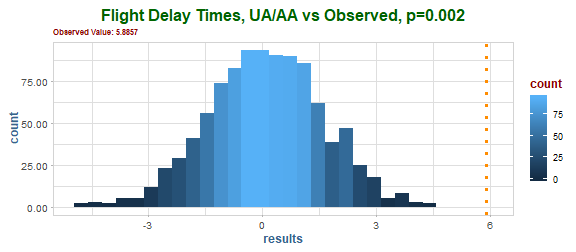
\includegraphics{03_permutation_testing_files/figure-latex/unnamed-chunk-7-1.png}

b.) The flights took place in May and June of 2009. Conduct a two-sided
permutation test to see if the differences in mean delay times between
two months is statistically significant.

\begin{Shaded}
\begin{Highlighting}[]
\NormalTok{Flights[, .(}\DataTypeTok{Delay =} \KeywordTok{mean}\NormalTok{(Delay)), by =}\StringTok{ }\NormalTok{Month]}
\end{Highlighting}
\end{Shaded}

\begin{verbatim}
   Month     Delay
1:   May  8.884442
2:  June 14.547783
\end{verbatim}

\begin{Shaded}
\begin{Highlighting}[]
\NormalTok{observed <-}\StringTok{ }\KeywordTok{mean}\NormalTok{(Flights[Month }\OperatorTok{==}\StringTok{ "May"}\NormalTok{]}\OperatorTok{$}\NormalTok{Delay) }\OperatorTok{-}\StringTok{ }\KeywordTok{mean}\NormalTok{(Flights[Month }\OperatorTok{==}\StringTok{ "June"}\NormalTok{]}\OperatorTok{$}\NormalTok{Delay)}

\NormalTok{N <-}\StringTok{ }\FloatTok{10e2} \OperatorTok{-}\StringTok{ }\DecValTok{1}
\NormalTok{results <-}\StringTok{ }\KeywordTok{numeric}\NormalTok{(N)}

\ControlFlowTok{for}\NormalTok{(i }\ControlFlowTok{in} \DecValTok{1}\OperatorTok{:}\NormalTok{N)}
\NormalTok{\{}
\NormalTok{   index <-}\StringTok{ }\KeywordTok{sample}\NormalTok{(}\KeywordTok{nrow}\NormalTok{(Flights), }\KeywordTok{nrow}\NormalTok{(Flights[Month }\OperatorTok{==}\StringTok{ "May"}\NormalTok{]), }\DataTypeTok{replace =}\NormalTok{ F)}
\NormalTok{   results[i] =}\StringTok{ }\KeywordTok{mean}\NormalTok{(Flights[index]}\OperatorTok{$}\NormalTok{Delay) }\OperatorTok{-}\StringTok{ }\KeywordTok{mean}\NormalTok{(Flights[}\OperatorTok{-}\NormalTok{index]}\OperatorTok{$}\NormalTok{Delay)}
\NormalTok{\}}

\CommentTok{# two-sided test}

\NormalTok{p <-}\StringTok{ }\DecValTok{2} \OperatorTok{*}\StringTok{ }\NormalTok{(}\KeywordTok{sum}\NormalTok{(results[results }\OperatorTok{<=}\StringTok{ }\NormalTok{observed]) }\OperatorTok{+}\StringTok{ }\DecValTok{1}\NormalTok{) }\OperatorTok{/}\StringTok{ }\NormalTok{( N }\OperatorTok{+}\StringTok{ }\DecValTok{1}\NormalTok{)}
\NormalTok{v <-}\StringTok{ }\NormalTok{p}\OperatorTok{*}\NormalTok{(}\DecValTok{1} \OperatorTok{-}\StringTok{ }\NormalTok{p) }\OperatorTok{/}\StringTok{ }\NormalTok{( N }\OperatorTok{+}\StringTok{ }\DecValTok{1}\NormalTok{ )}

\KeywordTok{ggplot}\NormalTok{(}\KeywordTok{data.table}\NormalTok{(results)) }\OperatorTok{+}
\StringTok{   }\KeywordTok{geom_histogram}\NormalTok{(}\KeywordTok{aes}\NormalTok{(results, }\DataTypeTok{fill =}\NormalTok{ ..count..), }\DataTypeTok{bins =} \DecValTok{30}\NormalTok{) }\OperatorTok{+}
\StringTok{   }\KeywordTok{geom_vline}\NormalTok{(}\DataTypeTok{xintercept =}\NormalTok{ observed, }\DataTypeTok{col =} \StringTok{"darkorange"}\NormalTok{, }\DataTypeTok{linetype =} \DecValTok{3}\NormalTok{, }\DataTypeTok{lwd =} \FloatTok{1.2}\NormalTok{) }\OperatorTok{+}
\StringTok{   }\KeywordTok{scale_y_continuous}\NormalTok{(}\DataTypeTok{labels =}\NormalTok{ comma) }\OperatorTok{+}
\StringTok{   }\KeywordTok{labs}\NormalTok{(}\DataTypeTok{title =} \KeywordTok{paste0}\NormalTok{(}\StringTok{"Flight Delay Times, May/June, vs Observed, p="}\NormalTok{, }\KeywordTok{round}\NormalTok{(p, }\DecValTok{5}\NormalTok{)),}
        \DataTypeTok{subtitle =} \KeywordTok{paste0}\NormalTok{(}\StringTok{"Observed Value: "}\NormalTok{, }\KeywordTok{round}\NormalTok{(observed, }\DecValTok{4}\NormalTok{)))}
\end{Highlighting}
\end{Shaded}

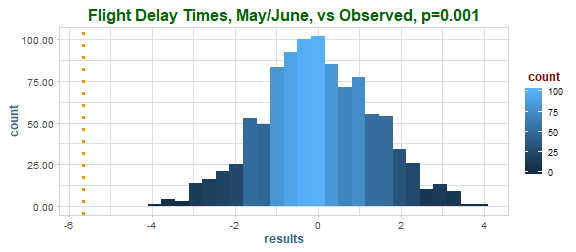
\includegraphics{03_permutation_testing_files/figure-latex/unnamed-chunk-8-1.png}

\hypertarget{section-5}{%
\subsection{3.6}\label{section-5}}

In the flight delays case study in Section 1.1, the data contains flight
delays for two airlines, American and United.

a.) Compute the proportion of times that each carrier's flight was
delays more than 20 min.

\begin{Shaded}
\begin{Highlighting}[]
\NormalTok{Flights[, .(}\DataTypeTok{Delay20 =} \KeywordTok{sum}\NormalTok{(Delay }\OperatorTok{>}\StringTok{ }\DecValTok{20}\NormalTok{) }\OperatorTok{/}\StringTok{ }\NormalTok{.N), by =}\StringTok{ }\NormalTok{Carrier]}
\end{Highlighting}
\end{Shaded}

\begin{verbatim}
   Carrier   Delay20
1:      UA 0.2128228
2:      AA 0.1693049
\end{verbatim}

\begin{Shaded}
\begin{Highlighting}[]
\NormalTok{observed <-}\StringTok{ }\KeywordTok{as.numeric}\NormalTok{(Flights[Carrier }\OperatorTok{==}\StringTok{ "UA"}\NormalTok{, .(}\DataTypeTok{Delay =} \KeywordTok{sum}\NormalTok{(Delay }\OperatorTok{>}\StringTok{ }\DecValTok{20}\NormalTok{)}\OperatorTok{/}\NormalTok{.N)] }\OperatorTok{-}\StringTok{ }\NormalTok{Flights[Carrier }\OperatorTok{==}\StringTok{ "AA"}\NormalTok{, .(}\DataTypeTok{Delay =} \KeywordTok{sum}\NormalTok{(Delay }\OperatorTok{>}\StringTok{ }\DecValTok{20}\NormalTok{)}\OperatorTok{/}\NormalTok{.N)])}

\NormalTok{N <-}\StringTok{ }\FloatTok{10e2} \OperatorTok{-}\StringTok{ }\DecValTok{1}
\NormalTok{results <-}\StringTok{ }\KeywordTok{numeric}\NormalTok{(N)}

\ControlFlowTok{for}\NormalTok{(i }\ControlFlowTok{in} \DecValTok{1}\OperatorTok{:}\NormalTok{N)}
\NormalTok{\{}
\NormalTok{   index <-}\StringTok{ }\KeywordTok{sample}\NormalTok{(}\KeywordTok{nrow}\NormalTok{(Flights), }\KeywordTok{nrow}\NormalTok{(Flights[Carrier }\OperatorTok{==}\StringTok{ "UA"}\NormalTok{]), }\DataTypeTok{replace =}\NormalTok{ F)}
\NormalTok{   results[i] <-}\StringTok{ }\KeywordTok{as.numeric}\NormalTok{(Flights[index, .(}\DataTypeTok{Delay =} \KeywordTok{sum}\NormalTok{(Delay }\OperatorTok{>}\StringTok{ }\DecValTok{20}\NormalTok{)}\OperatorTok{/}\NormalTok{.N)] }\OperatorTok{-}\StringTok{ }\NormalTok{Flights[}\OperatorTok{-}\NormalTok{index, .(}\DataTypeTok{Delay =} \KeywordTok{sum}\NormalTok{(Delay }\OperatorTok{>}\StringTok{ }\DecValTok{20}\NormalTok{)}\OperatorTok{/}\NormalTok{.N)])}
\NormalTok{\}}

\NormalTok{p <-}\StringTok{ }\DecValTok{2} \OperatorTok{*}\StringTok{ }\NormalTok{(}\KeywordTok{sum}\NormalTok{(results[results }\OperatorTok{>=}\StringTok{ }\NormalTok{observed]) }\OperatorTok{+}\StringTok{ }\DecValTok{1}\NormalTok{) }\OperatorTok{/}\StringTok{ }\NormalTok{( N }\OperatorTok{+}\StringTok{ }\DecValTok{1}\NormalTok{)}
\NormalTok{v <-}\StringTok{ }\NormalTok{p}\OperatorTok{*}\NormalTok{(}\DecValTok{1} \OperatorTok{-}\StringTok{ }\NormalTok{p) }\OperatorTok{/}\StringTok{ }\NormalTok{( N }\OperatorTok{+}\StringTok{ }\DecValTok{1}\NormalTok{ )}

\KeywordTok{ggplot}\NormalTok{(}\KeywordTok{data.table}\NormalTok{(results)) }\OperatorTok{+}
\StringTok{   }\KeywordTok{geom_histogram}\NormalTok{(}\KeywordTok{aes}\NormalTok{(results, }\DataTypeTok{fill =}\NormalTok{ ..count..), }\DataTypeTok{bins =} \DecValTok{30}\NormalTok{) }\OperatorTok{+}
\StringTok{   }\KeywordTok{geom_vline}\NormalTok{(}\DataTypeTok{xintercept =}\NormalTok{ observed, }\DataTypeTok{col =} \StringTok{"darkorange"}\NormalTok{, }\DataTypeTok{linetype =} \DecValTok{3}\NormalTok{, }\DataTypeTok{lwd =} \FloatTok{1.2}\NormalTok{) }\OperatorTok{+}
\StringTok{   }\KeywordTok{scale_y_continuous}\NormalTok{(}\DataTypeTok{labels =}\NormalTok{ comma) }\OperatorTok{+}
\StringTok{   }\KeywordTok{labs}\NormalTok{(}\DataTypeTok{title =} \KeywordTok{paste0}\NormalTok{(}\StringTok{"Flight Delay Times, Over 20 Minutes, vs Observed, p="}\NormalTok{, }\KeywordTok{round}\NormalTok{(p, }\DecValTok{5}\NormalTok{)), }
        \DataTypeTok{subtitle =} \KeywordTok{paste0}\NormalTok{(}\StringTok{"Observed Value: "}\NormalTok{, }\KeywordTok{round}\NormalTok{(observed, }\DecValTok{4}\NormalTok{)))}
\end{Highlighting}
\end{Shaded}

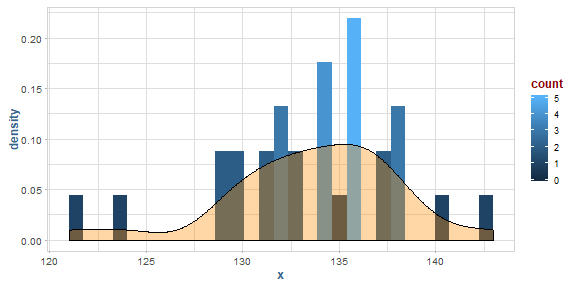
\includegraphics{03_permutation_testing_files/figure-latex/unnamed-chunk-9-1.png}

\begin{itemize}
\tightlist
\item
  Conduct a two-sided test to see if the difference in these proportions
  is statistically significant.
\end{itemize}

\textbf{Answer}: There is statistical significance with a P-value
\textless{} 0.0001.

b.) Compute the variance in the flight delay lengths for each carrier.

\begin{Shaded}
\begin{Highlighting}[]
\NormalTok{Flights[, .(}\DataTypeTok{Variance =} \KeywordTok{var}\NormalTok{(Delay)), by =}\StringTok{ }\NormalTok{Carrier]}
\end{Highlighting}
\end{Shaded}

\begin{verbatim}
   Carrier Variance
1:      UA 2037.525
2:      AA 1606.457
\end{verbatim}

\begin{Shaded}
\begin{Highlighting}[]
\NormalTok{observed <-}\StringTok{ }\KeywordTok{var}\NormalTok{(Flights[Carrier }\OperatorTok{==}\StringTok{ "UA"}\NormalTok{]}\OperatorTok{$}\NormalTok{Delay) }\OperatorTok{-}\StringTok{ }\KeywordTok{var}\NormalTok{(Flights[Carrier }\OperatorTok{==}\StringTok{ "AA"}\NormalTok{]}\OperatorTok{$}\NormalTok{Delay)}

\NormalTok{N <-}\StringTok{ }\FloatTok{10e2} \OperatorTok{-}\StringTok{ }\DecValTok{1}
\NormalTok{results <-}\StringTok{ }\KeywordTok{numeric}\NormalTok{(N)}

\ControlFlowTok{for}\NormalTok{(i }\ControlFlowTok{in} \DecValTok{1}\OperatorTok{:}\NormalTok{N)}
\NormalTok{\{}
\NormalTok{   index <-}\StringTok{ }\KeywordTok{sample}\NormalTok{(}\KeywordTok{nrow}\NormalTok{(Flights), }\KeywordTok{nrow}\NormalTok{(Flights[Carrier }\OperatorTok{==}\StringTok{ "UA"}\NormalTok{]), }\DataTypeTok{replace =}\NormalTok{ F)}
\NormalTok{   results[i] <-}\StringTok{ }\KeywordTok{var}\NormalTok{(Flights[index]}\OperatorTok{$}\NormalTok{Delay) }\OperatorTok{-}\StringTok{ }\KeywordTok{var}\NormalTok{(Flights[}\OperatorTok{-}\NormalTok{index]}\OperatorTok{$}\NormalTok{Delay)}
\NormalTok{\}}

\NormalTok{p <-}\StringTok{ }\KeywordTok{min}\NormalTok{(}\DecValTok{1}\NormalTok{, }\DecValTok{2} \OperatorTok{*}\StringTok{ }\NormalTok{(}\KeywordTok{sum}\NormalTok{(results[results }\OperatorTok{>=}\StringTok{ }\NormalTok{observed]) }\OperatorTok{+}\StringTok{ }\DecValTok{1}\NormalTok{) }\OperatorTok{/}\StringTok{ }\NormalTok{( N }\OperatorTok{+}\StringTok{ }\DecValTok{1}\NormalTok{))}
\NormalTok{v <-}\StringTok{ }\NormalTok{p}\OperatorTok{*}\NormalTok{(}\DecValTok{1} \OperatorTok{-}\StringTok{ }\NormalTok{p) }\OperatorTok{/}\StringTok{ }\NormalTok{( N }\OperatorTok{+}\StringTok{ }\DecValTok{1}\NormalTok{ )}

\KeywordTok{ggplot}\NormalTok{(}\KeywordTok{data.table}\NormalTok{(results)) }\OperatorTok{+}
\StringTok{   }\KeywordTok{geom_histogram}\NormalTok{(}\KeywordTok{aes}\NormalTok{(results, }\DataTypeTok{fill =}\NormalTok{ ..count..), }\DataTypeTok{bins =} \DecValTok{30}\NormalTok{) }\OperatorTok{+}
\StringTok{   }\KeywordTok{geom_vline}\NormalTok{(}\DataTypeTok{xintercept =}\NormalTok{ observed, }\DataTypeTok{col =} \StringTok{"darkorange"}\NormalTok{, }\DataTypeTok{linetype =} \DecValTok{3}\NormalTok{, }\DataTypeTok{lwd =} \FloatTok{1.2}\NormalTok{) }\OperatorTok{+}
\StringTok{   }\KeywordTok{scale_y_continuous}\NormalTok{(}\DataTypeTok{labels =}\NormalTok{ comma) }\OperatorTok{+}
\StringTok{   }\KeywordTok{labs}\NormalTok{(}\DataTypeTok{title =} \KeywordTok{paste0}\NormalTok{(}\StringTok{"Flight Delay Time Variance, vs Observed, p="}\NormalTok{, }\KeywordTok{round}\NormalTok{(p, }\DecValTok{5}\NormalTok{)), }
        \DataTypeTok{subtitle =} \KeywordTok{paste0}\NormalTok{(}\StringTok{"Observed Value: "}\NormalTok{, }\KeywordTok{round}\NormalTok{(observed, }\DecValTok{4}\NormalTok{)))}
\end{Highlighting}
\end{Shaded}

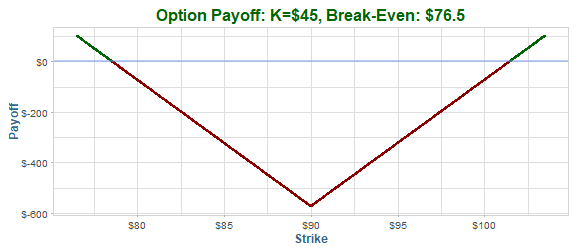
\includegraphics{03_permutation_testing_files/figure-latex/unnamed-chunk-10-1.png}

\begin{itemize}
\tightlist
\item
  Conduct a test to see if the variance for United Airlines differes
  from that of American Airlines.
\end{itemize}

\textbf{Answer}: There does not appear to be a statistically significant
difference in the variance in delay times between airlines.

\newpage

\hypertarget{section-6}{%
\subsection{3.7}\label{section-6}}

In the flight delays case study in Section 1.1, repeat Excercise 3.5
part \textbf{(a)} using three test statistics,

\begin{itemize}
\tightlist
\item
  i.) The mean of the United Airline delay times
\item
  ii.) The sum of the United Airline delay times
\item
  iii.) The difference in the means
\end{itemize}

Compare the P-values.

Make sure all three test statistics are computed within the same
\textbf{for} loop.

What do you observe?

\begin{Shaded}
\begin{Highlighting}[]
\NormalTok{UA.Delay <-}\StringTok{ }\NormalTok{Flights[Carrier }\OperatorTok{==}\StringTok{ "UA"}\NormalTok{]}\OperatorTok{$}\NormalTok{Delay}
\NormalTok{AA.Delay <-}\StringTok{ }\NormalTok{Flights[Carrier }\OperatorTok{==}\StringTok{ "AA"}\NormalTok{]}\OperatorTok{$}\NormalTok{Delay}

\NormalTok{observed.mean <-}\StringTok{ }\KeywordTok{mean}\NormalTok{(UA.Delay)}
\NormalTok{observed.sum <-}\StringTok{ }\KeywordTok{sum}\NormalTok{(UA.Delay)}
\NormalTok{observed.diff <-}\StringTok{ }\KeywordTok{mean}\NormalTok{(UA.Delay) }\OperatorTok{-}\StringTok{ }\KeywordTok{mean}\NormalTok{(AA.Delay)}

\NormalTok{N <-}\StringTok{ }\FloatTok{10e2} \OperatorTok{-}\StringTok{ }\DecValTok{1}
\NormalTok{results <-}\StringTok{ }\KeywordTok{matrix}\NormalTok{(}\DataTypeTok{nrow =}\NormalTok{ N, }\DataTypeTok{ncol =} \DecValTok{3}\NormalTok{)}

\ControlFlowTok{for}\NormalTok{(i }\ControlFlowTok{in} \DecValTok{1}\OperatorTok{:}\NormalTok{N)}
\NormalTok{\{}
\NormalTok{   index <-}\StringTok{ }\KeywordTok{sample}\NormalTok{(}\KeywordTok{nrow}\NormalTok{(Flights), }\KeywordTok{length}\NormalTok{(UA.Delay), }\DataTypeTok{replace =}\NormalTok{ F)}

\NormalTok{   results[i, }\DecValTok{1}\NormalTok{] <-}\StringTok{ }\KeywordTok{mean}\NormalTok{(Flights[index]}\OperatorTok{$}\NormalTok{Delay)}
\NormalTok{   results[i, }\DecValTok{2}\NormalTok{] <-}\StringTok{ }\KeywordTok{sum}\NormalTok{(Flights[index]}\OperatorTok{$}\NormalTok{Delay)}
\NormalTok{   results[i, }\DecValTok{3}\NormalTok{] <-}\StringTok{ }\KeywordTok{mean}\NormalTok{(Flights[index]}\OperatorTok{$}\NormalTok{Delay) }\OperatorTok{-}\StringTok{ }\KeywordTok{mean}\NormalTok{(Flights[}\OperatorTok{-}\NormalTok{index]}\OperatorTok{$}\NormalTok{Delay)}
\NormalTok{\}}

\NormalTok{dt.results <-}\StringTok{ }\KeywordTok{data.table}\NormalTok{(results)}
\KeywordTok{colnames}\NormalTok{(dt.results) <-}\StringTok{ }\KeywordTok{c}\NormalTok{(}\StringTok{"Mean"}\NormalTok{, }\StringTok{"Sum"}\NormalTok{, }\StringTok{"MeanDiff"}\NormalTok{)}

\NormalTok{p.mean <-}\StringTok{ }\NormalTok{( }\KeywordTok{sum}\NormalTok{( dt.results}\OperatorTok{$}\NormalTok{Mean }\OperatorTok{>=}\StringTok{ }\NormalTok{observed.mean ) }\OperatorTok{+}\StringTok{ }\DecValTok{1}\NormalTok{ ) }\OperatorTok{/}\StringTok{ }\NormalTok{( N }\OperatorTok{+}\StringTok{ }\DecValTok{1}\NormalTok{)}
\NormalTok{p.sum <-}\StringTok{ }\NormalTok{( }\KeywordTok{sum}\NormalTok{(dt.results}\OperatorTok{$}\NormalTok{Sum }\OperatorTok{>=}\StringTok{ }\NormalTok{observed.sum) }\OperatorTok{+}\StringTok{ }\DecValTok{1}\NormalTok{) }\OperatorTok{/}\StringTok{ }\NormalTok{( N }\OperatorTok{+}\StringTok{ }\DecValTok{1}\NormalTok{ )}
\NormalTok{p.diff <-}\StringTok{ }\NormalTok{( }\KeywordTok{sum}\NormalTok{(dt.results}\OperatorTok{$}\NormalTok{MeanDiff }\OperatorTok{>=}\StringTok{ }\NormalTok{observed.diff) }\OperatorTok{+}\StringTok{ }\DecValTok{1}\NormalTok{) }\OperatorTok{/}\StringTok{ }\NormalTok{( N }\OperatorTok{+}\StringTok{ }\DecValTok{1}\NormalTok{)}

\NormalTok{p1 <-}\StringTok{ }\KeywordTok{ggplot}\NormalTok{(dt.results) }\OperatorTok{+}
\StringTok{   }\KeywordTok{geom_histogram}\NormalTok{(}\KeywordTok{aes}\NormalTok{(Mean, }\DataTypeTok{fill =}\NormalTok{ ..count..), }\DataTypeTok{bins =} \DecValTok{30}\NormalTok{) }\OperatorTok{+}
\StringTok{   }\KeywordTok{geom_vline}\NormalTok{(}\DataTypeTok{xintercept =}\NormalTok{ observed.mean, }\DataTypeTok{col =} \StringTok{"darkorange"}\NormalTok{, }\DataTypeTok{lwd =} \FloatTok{1.2}\NormalTok{, }\DataTypeTok{linetype =} \DecValTok{3}\NormalTok{) }\OperatorTok{+}
\StringTok{   }\KeywordTok{scale_y_continuous}\NormalTok{(}\DataTypeTok{labels =}\NormalTok{ comma) }\OperatorTok{+}
\StringTok{   }\KeywordTok{labs}\NormalTok{(}\DataTypeTok{title =} \KeywordTok{paste0}\NormalTok{(}\StringTok{"United Airlines - Mean Delay Time vs Observed, p="}\NormalTok{, }\KeywordTok{round}\NormalTok{(p.mean, }\DecValTok{5}\NormalTok{)), }
        \DataTypeTok{subtitle =} \KeywordTok{paste0}\NormalTok{(}\StringTok{"Observed Value: "}\NormalTok{, }\KeywordTok{round}\NormalTok{(observed.mean, }\DecValTok{4}\NormalTok{)))}

\NormalTok{p2 <-}\StringTok{ }\KeywordTok{ggplot}\NormalTok{(dt.results) }\OperatorTok{+}
\StringTok{   }\KeywordTok{geom_histogram}\NormalTok{(}\KeywordTok{aes}\NormalTok{(Sum, }\DataTypeTok{fill =}\NormalTok{ ..count..), }\DataTypeTok{bins =} \DecValTok{30}\NormalTok{) }\OperatorTok{+}
\StringTok{   }\KeywordTok{geom_vline}\NormalTok{(}\DataTypeTok{xintercept =}\NormalTok{ observed.sum, }\DataTypeTok{col =} \StringTok{"darkorange"}\NormalTok{, }\DataTypeTok{lwd =} \FloatTok{1.2}\NormalTok{, }\DataTypeTok{linetype =} \DecValTok{3}\NormalTok{) }\OperatorTok{+}
\StringTok{   }\KeywordTok{scale_y_continuous}\NormalTok{(}\DataTypeTok{labels =}\NormalTok{ comma) }\OperatorTok{+}
\StringTok{   }\KeywordTok{labs}\NormalTok{(}\DataTypeTok{title =} \KeywordTok{paste0}\NormalTok{(}\StringTok{"United Airlines - Sum Delay Time vs Observed, p="}\NormalTok{, }\KeywordTok{round}\NormalTok{(p.sum, }\DecValTok{5}\NormalTok{)), }
        \DataTypeTok{subtitle =} \KeywordTok{paste0}\NormalTok{(}\StringTok{"Observed Value: "}\NormalTok{, }\KeywordTok{round}\NormalTok{(observed.sum, }\DecValTok{4}\NormalTok{)))}

\NormalTok{p3 <-}\StringTok{ }\KeywordTok{ggplot}\NormalTok{(dt.results) }\OperatorTok{+}
\StringTok{   }\KeywordTok{geom_histogram}\NormalTok{(}\KeywordTok{aes}\NormalTok{(MeanDiff, }\DataTypeTok{fill =}\NormalTok{ ..count..), }\DataTypeTok{bins =} \DecValTok{30}\NormalTok{) }\OperatorTok{+}
\StringTok{   }\KeywordTok{geom_vline}\NormalTok{(}\DataTypeTok{xintercept =}\NormalTok{ observed.diff, }\DataTypeTok{col =} \StringTok{"darkorange"}\NormalTok{, }\DataTypeTok{lwd =} \FloatTok{1.2}\NormalTok{, }\DataTypeTok{linetype =} \DecValTok{3}\NormalTok{) }\OperatorTok{+}
\StringTok{   }\KeywordTok{scale_y_continuous}\NormalTok{(}\DataTypeTok{labels =}\NormalTok{ comma) }\OperatorTok{+}
\StringTok{   }\KeywordTok{labs}\NormalTok{(}\DataTypeTok{title =} \KeywordTok{paste0}\NormalTok{(}\StringTok{"Mean Delay Time Difference vs Observed, p="}\NormalTok{, }\KeywordTok{round}\NormalTok{(p.diff, }\DecValTok{5}\NormalTok{)), }
        \DataTypeTok{subtitle =} \KeywordTok{paste0}\NormalTok{(}\StringTok{"Observed Value: "}\NormalTok{, }\KeywordTok{round}\NormalTok{(observed.diff, }\DecValTok{4}\NormalTok{)))}

\KeywordTok{grid.arrange}\NormalTok{(p1, p2, p3, }\DataTypeTok{nrow =} \DecValTok{3}\NormalTok{)}
\end{Highlighting}
\end{Shaded}

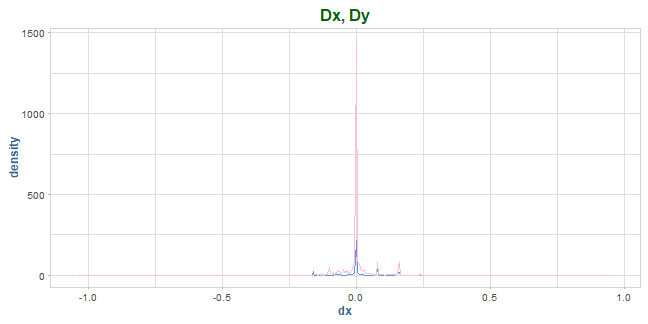
\includegraphics{03_permutation_testing_files/figure-latex/unnamed-chunk-11-1.png}

\newpage

\hypertarget{section-7}{%
\subsection{3.8}\label{section-7}}

In the flight delays case study in Section 1.1,

a.) Find the trimmed mean of the delay times for United Airlines and
American Airlines.

\begin{Shaded}
\begin{Highlighting}[]
\NormalTok{trim.amount <-}\StringTok{ }\FloatTok{.25}
\NormalTok{UA.trimmed <-}\StringTok{ }\KeywordTok{mean}\NormalTok{(UA.Delay, }\DataTypeTok{trim =}\NormalTok{ trim.amount)}
\NormalTok{AA.trimmed <-}\StringTok{ }\KeywordTok{mean}\NormalTok{(AA.Delay, }\DataTypeTok{trim =}\NormalTok{ trim.amount)}

\NormalTok{observed <-}\StringTok{ }\NormalTok{UA.trimmed }\OperatorTok{-}\StringTok{ }\NormalTok{AA.trimmed}

\KeywordTok{pretty_kable}\NormalTok{(}\KeywordTok{data.table}\NormalTok{( }\DataTypeTok{UA =}\NormalTok{ UA.trimmed, }\DataTypeTok{AA =}\NormalTok{ AA.trimmed), }\StringTok{"Trimmed Means"}\NormalTok{)}
\end{Highlighting}
\end{Shaded}

\begin{table}[!h]

\caption{\label{tab:unnamed-chunk-12}Trimmed Means}
\centering
\begin{tabular}[t]{r|r}
\hline
UA & AA\\
\hline
-0.8 & -2.57\\
\hline
\end{tabular}
\end{table}

b.) Conduct a two-sided test to see if the difference in trimmed means
is statistically significant.

\begin{Shaded}
\begin{Highlighting}[]
\NormalTok{N <-}\StringTok{ }\FloatTok{10e2} \OperatorTok{-}\StringTok{ }\DecValTok{1}
\NormalTok{results <-}\StringTok{ }\KeywordTok{numeric}\NormalTok{(N)}

\ControlFlowTok{for}\NormalTok{(i }\ControlFlowTok{in} \DecValTok{1}\OperatorTok{:}\NormalTok{N)}
\NormalTok{\{}
\NormalTok{   index <-}\StringTok{ }\KeywordTok{sample}\NormalTok{(}\KeywordTok{nrow}\NormalTok{(Flights), }\KeywordTok{nrow}\NormalTok{(Flights[Carrier }\OperatorTok{==}\StringTok{ "UA"}\NormalTok{]), }\DataTypeTok{replace =}\NormalTok{ F)}
\NormalTok{   results[i] <-}\StringTok{ }\KeywordTok{mean}\NormalTok{(Flights[index]}\OperatorTok{$}\NormalTok{Delay, }\DataTypeTok{trim =}\NormalTok{ trim.amount) }\OperatorTok{-}\StringTok{ }\KeywordTok{mean}\NormalTok{(Flights[}\OperatorTok{-}\NormalTok{index]}\OperatorTok{$}\NormalTok{Delay, }\DataTypeTok{trim =}\NormalTok{ trim.amount)}
\NormalTok{\}}

\NormalTok{p <-}\StringTok{ }\KeywordTok{min}\NormalTok{(}\DecValTok{1}\NormalTok{, }\DecValTok{2} \OperatorTok{*}\StringTok{ }\NormalTok{(}\KeywordTok{sum}\NormalTok{(results[results }\OperatorTok{>=}\StringTok{ }\NormalTok{observed]) }\OperatorTok{+}\StringTok{ }\DecValTok{1}\NormalTok{) }\OperatorTok{/}\StringTok{ }\NormalTok{( N }\OperatorTok{+}\StringTok{ }\DecValTok{1}\NormalTok{))}
\NormalTok{v <-}\StringTok{ }\NormalTok{p}\OperatorTok{*}\NormalTok{(}\DecValTok{1} \OperatorTok{-}\StringTok{ }\NormalTok{p) }\OperatorTok{/}\StringTok{ }\NormalTok{( N }\OperatorTok{+}\StringTok{ }\DecValTok{1}\NormalTok{ )}

\KeywordTok{ggplot}\NormalTok{(}\KeywordTok{data.table}\NormalTok{(results)) }\OperatorTok{+}
\StringTok{   }\KeywordTok{geom_histogram}\NormalTok{(}\KeywordTok{aes}\NormalTok{(results, }\DataTypeTok{fill =}\NormalTok{ ..count..), }\DataTypeTok{bins =} \DecValTok{30}\NormalTok{) }\OperatorTok{+}
\StringTok{   }\KeywordTok{geom_vline}\NormalTok{(}\DataTypeTok{xintercept =}\NormalTok{ observed, }\DataTypeTok{col =} \StringTok{"darkorange"}\NormalTok{, }\DataTypeTok{linetype =} \DecValTok{3}\NormalTok{, }\DataTypeTok{lwd =} \FloatTok{1.2}\NormalTok{) }\OperatorTok{+}
\StringTok{   }\KeywordTok{scale_y_continuous}\NormalTok{(}\DataTypeTok{labels =}\NormalTok{ comma) }\OperatorTok{+}
\StringTok{   }\KeywordTok{labs}\NormalTok{(}\DataTypeTok{title =} \KeywordTok{paste0}\NormalTok{(}\StringTok{"Flight Delay Time Trimmed Mean vs Observed, p="}\NormalTok{, }\KeywordTok{round}\NormalTok{(p, }\DecValTok{5}\NormalTok{)), }
        \DataTypeTok{subtitle =} \KeywordTok{paste0}\NormalTok{(}\StringTok{"Observed Value: "}\NormalTok{, }\KeywordTok{round}\NormalTok{(observed, }\DecValTok{4}\NormalTok{)))}
\end{Highlighting}
\end{Shaded}

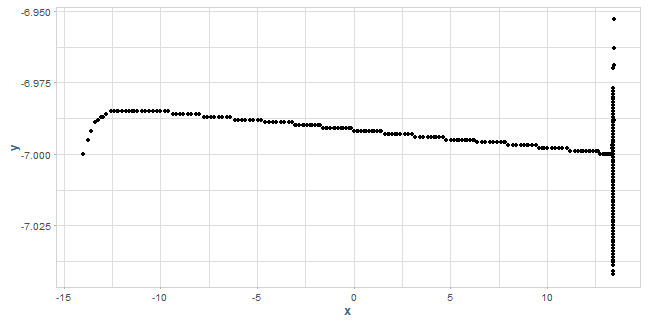
\includegraphics{03_permutation_testing_files/figure-latex/unnamed-chunk-13-1.png}

\hypertarget{section-8}{%
\subsection{3.9}\label{section-8}}

In the flight delays case study in Section 1.1,

a.) Compute the proportion of times the flights in May and in June were
delayed more than 20 min.

\begin{Shaded}
\begin{Highlighting}[]
\NormalTok{delay20_month <-}\StringTok{ }\NormalTok{Flights[, .(}\DataTypeTok{Delay20 =} \KeywordTok{sum}\NormalTok{(Delay }\OperatorTok{>}\StringTok{ }\DecValTok{20}\NormalTok{) }\OperatorTok{/}\StringTok{ }\NormalTok{.N), by =}\StringTok{ }\NormalTok{Month]}

\KeywordTok{pretty_kable}\NormalTok{(delay20_month, }\StringTok{"Delayed by more than 20 min, by month"}\NormalTok{)}
\end{Highlighting}
\end{Shaded}

\begin{table}[!h]

\caption{\label{tab:unnamed-chunk-14}Delayed by more than 20 min, by month}
\centering
\begin{tabular}[t]{l|r}
\hline
Month & Delay20\\
\hline
May & 0.17\\
\hline
June & 0.20\\
\hline
\end{tabular}
\end{table}

Conduct a two-sided test for statistical significance.

\begin{Shaded}
\begin{Highlighting}[]
\NormalTok{observed <-}\StringTok{ }\NormalTok{delay20_month[Month }\OperatorTok{==}\StringTok{ "May"}\NormalTok{]}\OperatorTok{$}\NormalTok{Delay20 }\OperatorTok{-}\StringTok{ }\NormalTok{delay20_month[Month }\OperatorTok{==}\StringTok{ "June"}\NormalTok{]}\OperatorTok{$}\NormalTok{Delay20}

\NormalTok{N <-}\StringTok{ }\FloatTok{10e2} \OperatorTok{-}\StringTok{ }\DecValTok{1}
\NormalTok{results <-}\StringTok{ }\KeywordTok{numeric}\NormalTok{(N)}

\ControlFlowTok{for}\NormalTok{( i }\ControlFlowTok{in} \DecValTok{1}\OperatorTok{:}\NormalTok{N)}
\NormalTok{\{}
\NormalTok{   index <-}\StringTok{ }\KeywordTok{sample}\NormalTok{(}\KeywordTok{nrow}\NormalTok{(Flights), }\KeywordTok{nrow}\NormalTok{(Flights[Month }\OperatorTok{==}\StringTok{ "May"}\NormalTok{]), }\DataTypeTok{replace =}\NormalTok{ F)}
\NormalTok{   results[i] <-}\StringTok{ }\KeywordTok{as.numeric}\NormalTok{( Flights[index, .(}\DataTypeTok{Delay =} \KeywordTok{sum}\NormalTok{(Delay }\OperatorTok{>}\StringTok{ }\DecValTok{20}\NormalTok{) }\OperatorTok{/}\StringTok{ }\NormalTok{.N)] }\OperatorTok{-}\StringTok{ }\NormalTok{Flights[}\OperatorTok{-}\NormalTok{index, .(}\DataTypeTok{Delay =} \KeywordTok{sum}\NormalTok{(Delay }\OperatorTok{>}\StringTok{ }\DecValTok{20}\NormalTok{) }\OperatorTok{/}\StringTok{ }\NormalTok{.N)] )}
\NormalTok{\}}

\NormalTok{p <-}\StringTok{ }\KeywordTok{min}\NormalTok{(}\DecValTok{1}\NormalTok{, }\DecValTok{2} \OperatorTok{*}\StringTok{ }\NormalTok{(}\KeywordTok{sum}\NormalTok{(results[results }\OperatorTok{>=}\StringTok{ }\NormalTok{observed]) }\OperatorTok{+}\StringTok{ }\DecValTok{1}\NormalTok{) }\OperatorTok{/}\StringTok{ }\NormalTok{( N }\OperatorTok{+}\StringTok{ }\DecValTok{1}\NormalTok{))}
\NormalTok{v <-}\StringTok{ }\NormalTok{p}\OperatorTok{*}\NormalTok{(}\DecValTok{1} \OperatorTok{-}\StringTok{ }\NormalTok{p) }\OperatorTok{/}\StringTok{ }\NormalTok{( N }\OperatorTok{+}\StringTok{ }\DecValTok{1}\NormalTok{ )}
\end{Highlighting}
\end{Shaded}

P-value: 0.0017, which is statistically significant.

b.) Compute the ratio of the variances in the flight delay times in May
and in June.

\begin{Shaded}
\begin{Highlighting}[]
\NormalTok{observed <-}\StringTok{ }\KeywordTok{var}\NormalTok{(Flights[Month }\OperatorTok{==}\StringTok{ "May"}\NormalTok{]}\OperatorTok{$}\NormalTok{Delay) }\OperatorTok{-}\StringTok{ }\KeywordTok{var}\NormalTok{(Flights[Month }\OperatorTok{==}\StringTok{ "June"}\NormalTok{]}\OperatorTok{$}\NormalTok{Delay)}

\NormalTok{N <-}\StringTok{ }\FloatTok{10e2} \OperatorTok{-}\StringTok{ }\DecValTok{1}
\NormalTok{results <-}\StringTok{ }\KeywordTok{numeric}\NormalTok{(N)}

\ControlFlowTok{for}\NormalTok{( i }\ControlFlowTok{in} \DecValTok{1}\OperatorTok{:}\NormalTok{N)}
\NormalTok{\{}
\NormalTok{   index <-}\StringTok{ }\KeywordTok{sample}\NormalTok{(}\KeywordTok{nrow}\NormalTok{(Flights), }\KeywordTok{nrow}\NormalTok{(Flights[Month }\OperatorTok{==}\StringTok{ "May"}\NormalTok{]), }\DataTypeTok{replace =}\NormalTok{ F)}
\NormalTok{   results[i] <-}\StringTok{ }\KeywordTok{var}\NormalTok{( Flights[index, .(Delay)] ) }\OperatorTok{-}\StringTok{ }\KeywordTok{var}\NormalTok{( Flights[}\OperatorTok{-}\NormalTok{index, .(Delay)] )}
\NormalTok{\}}

\NormalTok{p <-}\StringTok{ }\KeywordTok{min}\NormalTok{(}\DecValTok{1}\NormalTok{, }\DecValTok{2} \OperatorTok{*}\StringTok{ }\NormalTok{(}\KeywordTok{sum}\NormalTok{(results[results }\OperatorTok{>=}\StringTok{ }\NormalTok{observed]) }\OperatorTok{+}\StringTok{ }\DecValTok{1}\NormalTok{) }\OperatorTok{/}\StringTok{ }\NormalTok{( N }\OperatorTok{+}\StringTok{ }\DecValTok{1}\NormalTok{))}
\NormalTok{v <-}\StringTok{ }\NormalTok{p}\OperatorTok{*}\NormalTok{(}\DecValTok{1} \OperatorTok{-}\StringTok{ }\NormalTok{p) }\OperatorTok{/}\StringTok{ }\NormalTok{( N }\OperatorTok{+}\StringTok{ }\DecValTok{1}\NormalTok{ )}
\end{Highlighting}
\end{Shaded}

Is this evidence that the true ratio is not equal to 1, or could this be
due to chance variability?

The variance appear to be due to random chance, so there does appear to
be a stastical significance between the two months.

Conduct a two-sided test to check.

P-value: \textbf{1}

\hypertarget{section-9}{%
\subsection{3.10}\label{section-9}}

In the black spruce case study in Section 1.10, seedlings were planted
in plots that were either subject to competition (from other plants), or
not.

Use the data set \emph{Spruce} to conduct a test to see if the mean
difference is how much the seedlings grow (in height) over the corse of
the study under these two treatments is stastically significant.

\begin{Shaded}
\begin{Highlighting}[]
\NormalTok{Spruce <-}\StringTok{ }\KeywordTok{data.table}\NormalTok{(}\KeywordTok{read.csv}\NormalTok{(}\KeywordTok{paste0}\NormalTok{(data.dir, }\StringTok{"Spruce.csv"}\NormalTok{),}
                               \DataTypeTok{header =}\NormalTok{ T))}

\NormalTok{observed <-}\StringTok{ }\KeywordTok{mean}\NormalTok{( Spruce[Competition }\OperatorTok{==}\StringTok{ "NC"}\NormalTok{]}\OperatorTok{$}\NormalTok{Ht.change ) }\OperatorTok{-}\StringTok{ }\KeywordTok{mean}\NormalTok{( Spruce[Competition }\OperatorTok{==}\StringTok{ "C"}\NormalTok{]}\OperatorTok{$}\NormalTok{Ht.change )}

\NormalTok{N <-}\StringTok{ }\FloatTok{10e2} \OperatorTok{-}\StringTok{ }\DecValTok{1}
\NormalTok{results <-}\StringTok{ }\KeywordTok{numeric}\NormalTok{(N)}

\ControlFlowTok{for}\NormalTok{(i }\ControlFlowTok{in} \DecValTok{1}\OperatorTok{:}\NormalTok{N)}
\NormalTok{\{}
\NormalTok{   index <-}\StringTok{ }\KeywordTok{sample}\NormalTok{(}\KeywordTok{nrow}\NormalTok{(Spruce), }\KeywordTok{nrow}\NormalTok{(Spruce[Competition }\OperatorTok{==}\StringTok{ "NC"}\NormalTok{]), }\DataTypeTok{replace =}\NormalTok{ F)}
\NormalTok{   resutls <-}\StringTok{ }\KeywordTok{mean}\NormalTok{( Spruce[index]}\OperatorTok{$}\NormalTok{Ht.change ) }\OperatorTok{-}\StringTok{ }\KeywordTok{mean}\NormalTok{( Spruce[}\OperatorTok{-}\NormalTok{index]}\OperatorTok{$}\NormalTok{Ht.change )}
\NormalTok{\}}

\NormalTok{p <-}\StringTok{ }\KeywordTok{min}\NormalTok{(}\DecValTok{1}\NormalTok{, }\DecValTok{2} \OperatorTok{*}\StringTok{ }\NormalTok{(}\KeywordTok{sum}\NormalTok{(results[results }\OperatorTok{>=}\StringTok{ }\NormalTok{observed]) }\OperatorTok{+}\StringTok{ }\DecValTok{1}\NormalTok{) }\OperatorTok{/}\StringTok{ }\NormalTok{( N }\OperatorTok{+}\StringTok{ }\DecValTok{1}\NormalTok{))}
\end{Highlighting}
\end{Shaded}

There is stastical significance in between the heights of the two groups
(Competition / No-competition).

P-value: \textbf{0.002}

\hypertarget{section-10}{%
\subsection{3.11}\label{section-10}}

The file \emph{Phillies2009} contains data from the 2009 season for the
baseball team the Philadelphia Phillies.

\begin{Shaded}
\begin{Highlighting}[]
\NormalTok{Phillies <-}\StringTok{ }\KeywordTok{data.table}\NormalTok{(}\KeywordTok{read.csv}\NormalTok{(}\KeywordTok{paste0}\NormalTok{(data.dir, }\StringTok{"Phillies2009.csv"}\NormalTok{),}
                               \DataTypeTok{header =}\NormalTok{ T))}
\end{Highlighting}
\end{Shaded}

a.) Compare the empirical distribution functions of the number of
strike-outs per game (\emph{StrikeOuts}) for games played at home and
games played away (\emph{Location}).

\begin{Shaded}
\begin{Highlighting}[]
\KeywordTok{ggplot}\NormalTok{(Phillies, }\KeywordTok{aes}\NormalTok{(StrikeOuts, }\DataTypeTok{color =}\NormalTok{ Location)) }\OperatorTok{+}
\StringTok{   }\KeywordTok{stat_ecdf}\NormalTok{(}\DataTypeTok{stat =} \StringTok{"point"}\NormalTok{) }\OperatorTok{+}
\StringTok{   }\KeywordTok{labs}\NormalTok{(}\DataTypeTok{title =} \StringTok{"Strike-outs / Game, by Location"}\NormalTok{, }\DataTypeTok{y =} \StringTok{"Percent"}\NormalTok{)}
\end{Highlighting}
\end{Shaded}

\begin{verbatim}
Warning: Ignoring unknown parameters: stat
\end{verbatim}

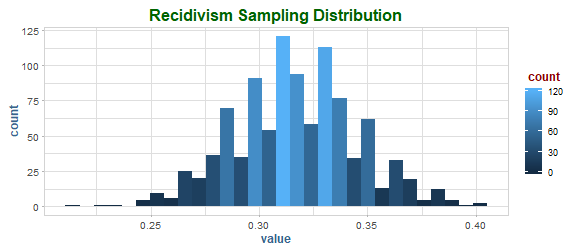
\includegraphics{03_permutation_testing_files/figure-latex/unnamed-chunk-19-1.png}

b.) Find the mean number of strike-outs per game for the home and the
away games.

\begin{Shaded}
\begin{Highlighting}[]
\NormalTok{strikeouts <-}\StringTok{ }\NormalTok{Phillies[, .(}\DataTypeTok{StrikeOuts =} \KeywordTok{mean}\NormalTok{(StrikeOuts)), by =}\StringTok{ }\NormalTok{Location]}

\KeywordTok{pretty_kable}\NormalTok{(strikeouts, }\StringTok{"StrikeOuts by Location"}\NormalTok{)}
\end{Highlighting}
\end{Shaded}

\begin{table}[!h]

\caption{\label{tab:unnamed-chunk-20}StrikeOuts by Location}
\centering
\begin{tabular}[t]{l|r}
\hline
Location & StrikeOuts\\
\hline
Home & 6.95\\
\hline
Away & 7.31\\
\hline
\end{tabular}
\end{table}

\begin{Shaded}
\begin{Highlighting}[]
\NormalTok{observed <-}\StringTok{ }\KeywordTok{mean}\NormalTok{(strikeouts[Location }\OperatorTok{==}\StringTok{ "Away"}\NormalTok{]}\OperatorTok{$}\NormalTok{StrikeOuts) }\OperatorTok{-}\StringTok{ }\KeywordTok{mean}\NormalTok{(strikeouts[Location }\OperatorTok{==}\StringTok{ "Home"}\NormalTok{]}\OperatorTok{$}\NormalTok{StrikeOuts)}
\end{Highlighting}
\end{Shaded}

c.) Perform a permutation tests to see if the differences in means is
statistically significant.

\begin{Shaded}
\begin{Highlighting}[]
\NormalTok{N <-}\StringTok{ }\FloatTok{10e2} \OperatorTok{-}\StringTok{ }\DecValTok{1}
\NormalTok{results <-}\StringTok{ }\KeywordTok{numeric}\NormalTok{(N)}

\ControlFlowTok{for}\NormalTok{( i }\ControlFlowTok{in} \DecValTok{1}\OperatorTok{:}\NormalTok{N)}
\NormalTok{\{}
\NormalTok{   index <-}\StringTok{ }\KeywordTok{sample}\NormalTok{(}\KeywordTok{nrow}\NormalTok{(Phillies), }\KeywordTok{nrow}\NormalTok{(Phillies[Location }\OperatorTok{==}\StringTok{ "Home"}\NormalTok{]), }\DataTypeTok{replace =}\NormalTok{ F)}
\NormalTok{   results[i] <-}\StringTok{ }\KeywordTok{mean}\NormalTok{(Phillies[index]}\OperatorTok{$}\NormalTok{StrikeOuts) }\OperatorTok{-}\StringTok{ }\KeywordTok{mean}\NormalTok{(Phillies[}\OperatorTok{-}\NormalTok{index]}\OperatorTok{$}\NormalTok{StrikeOuts)}
\NormalTok{\}}

\NormalTok{p <-}\StringTok{ }\KeywordTok{min}\NormalTok{(}\DecValTok{1}\NormalTok{, ( }\KeywordTok{sum}\NormalTok{(results }\OperatorTok{>=}\StringTok{ }\NormalTok{observed) }\OperatorTok{+}\StringTok{ }\DecValTok{1}\NormalTok{) }\OperatorTok{/}\StringTok{ }\NormalTok{( N }\OperatorTok{+}\StringTok{ }\DecValTok{1}\NormalTok{) )}
\end{Highlighting}
\end{Shaded}

There does not appear to be a statistically significat relationship
between the number of home and away strikeouts.

P-value: \textbf{0.192}

\hypertarget{section-11}{%
\subsection{3.12}\label{section-11}}

In the Iowa recidivism case study in Section 1.4, offenders had
originally been convicted of either a felony or misdemenor.

\begin{Shaded}
\begin{Highlighting}[]
\NormalTok{Recidivism <-}\StringTok{ }\KeywordTok{data.table}\NormalTok{(}\KeywordTok{read.csv}\NormalTok{(}\KeywordTok{paste0}\NormalTok{(data.dir, }\StringTok{"Recidivism.csv"}\NormalTok{),}
                               \DataTypeTok{header =}\NormalTok{ T))}
\end{Highlighting}
\end{Shaded}

a.) Use R to create a table displaying the proportion of felons who
recidivated and the propportion of those convictted of a misdemeanor who
recidivated.

\begin{Shaded}
\begin{Highlighting}[]
\NormalTok{Recidivism[, Recidivated }\OperatorTok{:}\ErrorTok{=}\StringTok{ }\KeywordTok{is.na}\NormalTok{(Days)]}

\NormalTok{Recidivated <-}\StringTok{ }\NormalTok{Recidivism[, .(}\DataTypeTok{RecidPct =} \KeywordTok{sum}\NormalTok{(Recidivated) }\OperatorTok{/}\StringTok{ }\NormalTok{.N), by =}\StringTok{ }\NormalTok{Offense]}

\KeywordTok{pretty_kable}\NormalTok{(Recidivated, }\StringTok{"Recidivated"}\NormalTok{)}
\end{Highlighting}
\end{Shaded}

\begin{table}[!h]

\caption{\label{tab:unnamed-chunk-23}Recidivated}
\centering
\begin{tabular}[t]{l|r}
\hline
Offense & RecidPct\\
\hline
Felony & 0.69\\
\hline
Misdemeanor & 0.67\\
\hline
\end{tabular}
\end{table}

b.) Determine whether or not the difference in recidivism proportions
computed in (a) is statistically significant.

\begin{Shaded}
\begin{Highlighting}[]
\NormalTok{observed <-}\StringTok{ }\KeywordTok{as.numeric}\NormalTok{( Recidivated[Offense }\OperatorTok{==}\StringTok{ "Felony"}\NormalTok{]}\OperatorTok{$}\NormalTok{RecidPct }\OperatorTok{-}\StringTok{ }\NormalTok{Recidivated[Offense }\OperatorTok{==}\StringTok{ "Misdemeanor"}\NormalTok{]}\OperatorTok{$}\NormalTok{RecidPct )}

\NormalTok{N <-}\StringTok{ }\FloatTok{10e2} \OperatorTok{-}\StringTok{ }\DecValTok{1}
\NormalTok{results <-}\StringTok{ }\KeywordTok{numeric}\NormalTok{(N)}

\ControlFlowTok{for}\NormalTok{( i }\ControlFlowTok{in} \DecValTok{1}\OperatorTok{:}\NormalTok{N )}
\NormalTok{\{}
\NormalTok{   index <-}\StringTok{ }\KeywordTok{sample}\NormalTok{(}\KeywordTok{nrow}\NormalTok{(Recidivism), }\KeywordTok{nrow}\NormalTok{(Recidivism[Offense }\OperatorTok{==}\StringTok{ "Felony"}\NormalTok{]), }\DataTypeTok{replace =}\NormalTok{ F)}
\NormalTok{   results[i] <-}\StringTok{ }\KeywordTok{as.numeric}\NormalTok{( Recidivism[index, .(}\DataTypeTok{Pct =} \KeywordTok{sum}\NormalTok{(Recidivated) }\OperatorTok{/}\StringTok{ }\NormalTok{.N)] }\OperatorTok{-}\StringTok{ }\NormalTok{Recidivism[}\OperatorTok{-}\NormalTok{index, .(}\DataTypeTok{Pct =} \KeywordTok{sum}\NormalTok{(Recidivated) }\OperatorTok{/}\StringTok{ }\NormalTok{.N)] )}
\NormalTok{\}}

\NormalTok{p <-}\StringTok{ }\NormalTok{( }\KeywordTok{sum}\NormalTok{(results }\OperatorTok{>=}\StringTok{ }\NormalTok{observed) }\OperatorTok{+}\StringTok{ }\DecValTok{1}\NormalTok{ ) }\OperatorTok{/}\StringTok{ }\NormalTok{( N }\OperatorTok{+}\StringTok{ }\DecValTok{1}\NormalTok{ )}
\end{Highlighting}
\end{Shaded}

It appears there is statistical significance in the recidivism rates
between felony and misdemeanor convictions.

P-value: 0.028

\hypertarget{section-12}{%
\subsection{3.13}\label{section-12}}

In the Iowa recidivism case study in Section 1.4, for those offenders
who recidivated, we have data on the number of days until they
reoffended.

For those offenders who did recidivate, determine if the difference in
the mean number of days (\textbf{Days}) until recidivism between those
under 25 years of age and those 25 years of age and older is
statistically significant.

\begin{Shaded}
\begin{Highlighting}[]
\NormalTok{Recid.Age25 <-}\StringTok{ }\NormalTok{Recidivism[, .(}\DataTypeTok{RecidDays =} \KeywordTok{mean}\NormalTok{(Days, }\DataTypeTok{na.rm =}\NormalTok{ T)), by =}\StringTok{ }\NormalTok{Age25]}

\KeywordTok{pretty_kable}\NormalTok{(Recid.Age25, }\StringTok{"Days Until Recidivism by Age ( < 25 < )"}\NormalTok{)}
\end{Highlighting}
\end{Shaded}

\begin{table}[!h]

\caption{\label{tab:unnamed-chunk-25}Days Until Recidivism by Age ( < 25 < )}
\centering
\begin{tabular}[t]{l|r}
\hline
Age25 & RecidDays\\
\hline
Under 25 & 449.07\\
\hline
Over 25 & 479.72\\
\hline
NA & NaN\\
\hline
\end{tabular}
\end{table}

\begin{Shaded}
\begin{Highlighting}[]
\NormalTok{observed <-}\StringTok{ }\KeywordTok{as.numeric}\NormalTok{( Recid.Age25[Age25 }\OperatorTok{==}\StringTok{ "Under 25"}\NormalTok{]}\OperatorTok{$}\NormalTok{RecidDays }\OperatorTok{-}\StringTok{ }\NormalTok{Recid.Age25[Age25 }\OperatorTok{==}\StringTok{ "Over 25"}\NormalTok{]}\OperatorTok{$}\NormalTok{RecidDays)}

\NormalTok{N <-}\StringTok{ }\FloatTok{10e2} \OperatorTok{-}\StringTok{ }\DecValTok{1}
\NormalTok{results <-}\StringTok{ }\KeywordTok{numeric}\NormalTok{(N)}

\ControlFlowTok{for}\NormalTok{( i }\ControlFlowTok{in} \DecValTok{1}\OperatorTok{:}\NormalTok{N )}
\NormalTok{\{}
\NormalTok{   index <-}\StringTok{ }\KeywordTok{sample}\NormalTok{(}\KeywordTok{nrow}\NormalTok{(Recidivism), }\KeywordTok{nrow}\NormalTok{(Recidivism[Age25 }\OperatorTok{==}\StringTok{ "Under 25"}\NormalTok{]), }\DataTypeTok{replace =}\NormalTok{ F)}
\NormalTok{   results[i] <-}\StringTok{ }\KeywordTok{mean}\NormalTok{(Recidivism[index]}\OperatorTok{$}\NormalTok{Days, }\DataTypeTok{na.rm =}\NormalTok{ T) }\OperatorTok{-}\StringTok{ }\KeywordTok{mean}\NormalTok{(Recidivism[}\OperatorTok{-}\NormalTok{index]}\OperatorTok{$}\NormalTok{Days, }\DataTypeTok{na.rm =}\NormalTok{ T)}
\NormalTok{\}}

\NormalTok{p <-}\StringTok{ }\KeywordTok{min}\NormalTok{(}\DecValTok{1}\NormalTok{, ( }\KeywordTok{sum}\NormalTok{(results }\OperatorTok{>=}\StringTok{ }\NormalTok{observed) }\OperatorTok{+}\StringTok{ }\DecValTok{1}\NormalTok{ ) }\OperatorTok{/}\StringTok{ }\NormalTok{( N }\OperatorTok{+}\StringTok{ }\DecValTok{1}\NormalTok{ ) )}
\end{Highlighting}
\end{Shaded}

There does not appear to be a statistical difference between the days
until recidivism by those over/under 25 years of age.

P-value: 0.998

\hypertarget{section-13}{%
\subsection{3.14}\label{section-13}}

Does chocolate ice cream have more calories than vanilla ice cream? The
data set \textbf{IceCream} contains calorie information for a sample of
brands of chocolate and vanilla ice cream.

\begin{Shaded}
\begin{Highlighting}[]
\NormalTok{IceCream <-}\StringTok{ }\KeywordTok{data.table}\NormalTok{(}\KeywordTok{read.csv}\NormalTok{(}\KeywordTok{paste0}\NormalTok{(data.dir, }\StringTok{"IceCream.csv"}\NormalTok{),}
                               \DataTypeTok{header =}\NormalTok{ T))}
\end{Highlighting}
\end{Shaded}

a.) Inspect the data set, then explain why this is an example of matched
pairs data.

\begin{Shaded}
\begin{Highlighting}[]
\KeywordTok{pretty_kable}\NormalTok{(IceCream, }\StringTok{"Ice Cream Data"}\NormalTok{)}
\end{Highlighting}
\end{Shaded}

\begin{table}[!h]

\caption{\label{tab:unnamed-chunk-27}Ice Cream Data}
\centering
\begin{tabular}[t]{l|r|r|r|r|r|r}
\hline
Brand & VanillaCalories & VanillaFat & VanillaSugar & ChocolateCalories & ChocolateFat & ChocolateSugar\\
\hline
Baskin Robbins & 260 & 16.0 & 26.0 & 260 & 14.0 & 31.0\\
\hline
Ben \& Jerry's & 240 & 16.0 & 19.0 & 260 & 16.0 & 22.0\\
\hline
Blue Bunny & 140 & 7.0 & 12.0 & 130 & 7.0 & 14.0\\
\hline
Breyers & 140 & 7.0 & 13.0 & 140 & 8.0 & 16.0\\
\hline
Brigham's & 190 & 12.0 & 17.0 & 200 & 12.0 & 18.0\\
\hline
Bulla & 234 & 13.5 & 21.8 & 266 & 15.0 & 22.6\\
\hline
Carvel & 240 & 14.0 & 21.0 & 250 & 13.0 & 25.0\\
\hline
Cass-Clay & 130 & 7.0 & 11.0 & 150 & 7.0 & 16.0\\
\hline
Chapman's & 120 & 6.0 & 11.0 & 120 & 5.0 & 12.0\\
\hline
Cold Stone & 270 & 15.5 & 23.0 & 264 & 16.2 & 23.6\\
\hline
Culver's & 222 & 13.0 & 19.0 & 205 & 10.0 & 20.0\\
\hline
Dairy Queen & 140 & 4.5 & 19.0 & 150 & 5.0 & 17.0\\
\hline
Dove & 240 & 15.0 & 20.0 & 290 & 17.0 & 27.0\\
\hline
Dreamery & 260 & 15.0 & 24.0 & 280 & 12.0 & 33.0\\
\hline
Edy's Grand & 140 & 8.0 & 13.0 & 150 & 8.0 & 15.0\\
\hline
Emack \& Bolio's & 160 & 9.0 & 12.0 & 170 & 9.0 & 13.0\\
\hline
Good Humor & 120 & 6.0 & 12.0 & 120 & 6.0 & 14.0\\
\hline
Graeter's & 260 & 16.0 & 24.0 & 260 & 16.0 & 24.0\\
\hline
Green and Black & 194 & 11.6 & 18.0 & 227 & 12.8 & 22.7\\
\hline
Green's & 150 & 8.0 & 17.0 & 140 & 8.0 & 15.0\\
\hline
Haagen Dazs & 270 & 18.0 & 21.0 & 270 & 18.0 & 21.0\\
\hline
Hershey's & 140 & 9.0 & 14.0 & 140 & 8.0 & 13.0\\
\hline
Hill Station & 226 & 15.6 & 16.8 & 235 & 14.3 & 21.2\\
\hline
Kemp's & 130 & 7.0 & 13.0 & 140 & 6.0 & 17.0\\
\hline
Klein's & 130 & 8.0 & 15.0 & 140 & 8.0 & 14.0\\
\hline
Oberweis Dairy & 307 & 21.0 & 23.0 & 320 & 21.0 & 19.0\\
\hline
Our Family & 130 & 7.0 & 11.0 & 130 & 6.0 & 15.0\\
\hline
Perry's & 140 & 8.0 & 15.0 & 140 & 7.0 & 15.0\\
\hline
Ronnybrook Farm & 240 & 16.0 & 20.0 & 260 & 19.0 & 21.0\\
\hline
Ruggles & 150 & 8.0 & 12.0 & 150 & 8.0 & 16.0\\
\hline
Sara Lee & 242 & 15.5 & 21.5 & 234 & 14.4 & 20.9\\
\hline
Schwan's & 140 & 7.0 & 12.0 & 140 & 7.0 & 12.0\\
\hline
Sheer Bliss & 300 & 19.0 & 27.0 & 320 & 19.0 & 29.0\\
\hline
Smith's & 150 & 8.0 & 13.0 & 150 & 8.0 & 13.0\\
\hline
Stonyfield Farm & 240 & 16.0 & 20.0 & 250 & 17.0 & 20.0\\
\hline
Tillamook & 160 & 9.0 & 10.0 & 170 & 9.0 & 13.0\\
\hline
Turkey Hill & 140 & 8.0 & 16.0 & 150 & 8.0 & 19.0\\
\hline
Value Choice & 130 & 6.0 & 12.0 & 130 & 6.0 & 15.0\\
\hline
Whitey's & 250 & 14.0 & 23.0 & 250 & 13.0 & 25.0\\
\hline
\end{tabular}
\end{table}

This data set is matched pairs becase there are multiple brands
associated with each flavor. They are not independent samples.

b.) Compute summary statistics of the number of calories for the two
flavors.

\begin{Shaded}
\begin{Highlighting}[]
\KeywordTok{pretty_kable}\NormalTok{(IceCream[, .(}\DataTypeTok{Vanilla =} \KeywordTok{mean}\NormalTok{(VanillaCalories), }\DataTypeTok{Chocolate =} \KeywordTok{mean}\NormalTok{(ChocolateCalories))], }
             \StringTok{"Ice cream Calories by Flavor"}\NormalTok{)}
\end{Highlighting}
\end{Shaded}

\begin{table}[!h]

\caption{\label{tab:unnamed-chunk-28}Ice cream Calories by Flavor}
\centering
\begin{tabular}[t]{r|r}
\hline
Vanilla & Chocolate\\
\hline
191.41 & 198.74\\
\hline
\end{tabular}
\end{table}

c.) Conduct a permutation tests to determine whether or not chocolate
ice cream has, on average, more calories than vanilla ice cream.

\begin{Shaded}
\begin{Highlighting}[]
\NormalTok{diff <-}\StringTok{ }\NormalTok{IceCream}\OperatorTok{$}\NormalTok{VanillaCalories }\OperatorTok{-}\StringTok{ }\NormalTok{IceCream}\OperatorTok{$}\NormalTok{ChocolateCalories}
\NormalTok{observed <-}\StringTok{ }\KeywordTok{mean}\NormalTok{(diff)}

\NormalTok{N <-}\StringTok{ }\FloatTok{10e2} \OperatorTok{-}\StringTok{ }\DecValTok{1}
\NormalTok{results <-}\StringTok{ }\KeywordTok{numeric}\NormalTok{(N)}

\ControlFlowTok{for}\NormalTok{( i }\ControlFlowTok{in} \DecValTok{1}\OperatorTok{:}\NormalTok{N )}
\NormalTok{\{}
\NormalTok{   Sign <-}\StringTok{ }\KeywordTok{sample}\NormalTok{(}\KeywordTok{c}\NormalTok{(}\OperatorTok{-}\DecValTok{1}\NormalTok{, }\DecValTok{1}\NormalTok{), }\KeywordTok{nrow}\NormalTok{(IceCream), }\DataTypeTok{replace =}\NormalTok{ T)}
\NormalTok{   diff2 <-}\StringTok{ }\NormalTok{Sign }\OperatorTok{*}\StringTok{ }\NormalTok{diff}
\NormalTok{   results[i] <-}\StringTok{ }\KeywordTok{mean}\NormalTok{(diff2)}
\NormalTok{\}}

\NormalTok{p <-}\StringTok{ }\NormalTok{( }\KeywordTok{sum}\NormalTok{( results }\OperatorTok{<=}\StringTok{ }\NormalTok{observed ) }\OperatorTok{+}\StringTok{ }\DecValTok{1}\NormalTok{ ) }\OperatorTok{/}\StringTok{ }\NormalTok{( N }\OperatorTok{+}\StringTok{ }\DecValTok{1}\NormalTok{ )}
\end{Highlighting}
\end{Shaded}

The data supports the claim that chocolate ice cream has more calories
than vanilla.

P-value: 0.002

\hypertarget{section-14}{%
\subsection{3.15}\label{section-14}}

Is there a difference in the price of groceries sold by the two
retailers Target and Walmart?

The data set Groceries contains a sample of grocery items and their
prices advertised on their respective web sites on one specific day.

\begin{Shaded}
\begin{Highlighting}[]
\NormalTok{Groceries <-}\StringTok{ }\KeywordTok{data.table}\NormalTok{(}\KeywordTok{read.csv}\NormalTok{(}\KeywordTok{paste0}\NormalTok{(data.dir, }\StringTok{"Groceries.csv"}\NormalTok{),}
                               \DataTypeTok{header =}\NormalTok{ T))}
\end{Highlighting}
\end{Shaded}

a.) Inspect the data set, then explain why this is an example of matched
pairs data.

\begin{Shaded}
\begin{Highlighting}[]
\KeywordTok{pretty_kable}\NormalTok{(Groceries, }\StringTok{"Target vs Walmart"}\NormalTok{)}
\end{Highlighting}
\end{Shaded}

\begin{table}[!h]

\caption{\label{tab:unnamed-chunk-31}Target vs Walmart}
\centering
\begin{tabular}[t]{l|l|r|r}
\hline
Product & Size & Target & Walmart\\
\hline
Kellogg NutriGrain Bars & 8 bars & 2.50 & 2.78\\
\hline
Quaker Oats Life Cereal  Original & 18oz & 3.19 & 6.01\\
\hline
General Mills Lucky Charms & 11.50z & 3.19 & 2.98\\
\hline
Quaker Oats Old Fashioned & 18oz & 2.82 & 2.68\\
\hline
Nabisco Oreo Cookies & 14.3oz & 2.99 & 2.98\\
\hline
Nabisco Chips Ahoy & 13oz & 2.64 & 1.98\\
\hline
Doritos Nacho Cheese Chips & 10oz & 3.99 & 2.50\\
\hline
Cheez-it Original Baked & 21oz & 4.79 & 4.79\\
\hline
Swiss Miss Hot Chocolate & 10 count & 1.49 & 1.28\\
\hline
Tazo Chai Classic Latte Black Tea & 32 oz & 3.49 & 2.98\\
\hline
Annie's Macaroni \& Cheese & 6oz & 1.79 & 1.72\\
\hline
Rice A Roni Chicken & 6.9oz & 1.00 & 1.00\\
\hline
Zatarain's Jambalaya Rice Mix & 8oz & 1.62 & 1.54\\
\hline
SPAM Original Lunch Meat & 12oz & 2.79 & 2.64\\
\hline
Campbell's Chicken Noodle Soup & 10.75oz & 0.99 & 1.58\\
\hline
Dinty Moore Hearty Meals Beef Stew & 15oz & 1.99 & 1.98\\
\hline
Hormel  Chili with Beans & 15oz & 1.94 & 1.88\\
\hline
Dole Pineapple Chunks & 20 oz & 1.59 & 1.47\\
\hline
Skippy Creamy Peanut Butter & 16.3oz & 2.59 & 2.58\\
\hline
Smucker's Strawberry Preserve & 18oz & 2.99 & 2.84\\
\hline
Heinz Tomato Ketchup & 32oz & 2.99 & 2.88\\
\hline
Near East Couscous Toasted Pine Nuts mix & 5.6oz & 2.12 & 1.98\\
\hline
Barilla Angel Hair Pasta & 16oz & 1.42 & 1.38\\
\hline
Betty Crocker Super Moist Chocolate Fudge Cake Mix & 15.25oz & 1.22 & 1.17\\
\hline
Kraft Jet-Puffed Marshmllows & 16oz & 1.99 & 1.96\\
\hline
Dunkin' Donuts Original Blend Medium Roast Ground Coffee & 12oz & 7.19 & 6.98\\
\hline
Dove Promises Milk Chocolate & 8.87oz & 3.19 & 3.50\\
\hline
Skittles & 41oz & 7.99 & 6.98\\
\hline
Vlasic Kosher Dill Pickle Spears & 24oz & 2.39 & 2.18\\
\hline
Vlasic Old Fashioned Sauerkraut & 32oz & 1.99 & 1.97\\
\hline
\end{tabular}
\end{table}

b.) Compute summary statistics of the prices for each store.

\begin{Shaded}
\begin{Highlighting}[]
\NormalTok{diff <-}\StringTok{ }\NormalTok{Groceries}\OperatorTok{$}\NormalTok{Target }\OperatorTok{-}\StringTok{ }\NormalTok{Groceries}\OperatorTok{$}\NormalTok{Walmart}

\NormalTok{observed <-}\StringTok{ }\KeywordTok{mean}\NormalTok{(diff)}
\end{Highlighting}
\end{Shaded}

Observed difference: \textbf{0.0566667}

c.) Conduct a permutation test to determine whether or not there is a
difference in the mean prices.

\begin{Shaded}
\begin{Highlighting}[]
\NormalTok{N <-}\StringTok{ }\FloatTok{10e2} \OperatorTok{-}\StringTok{ }\DecValTok{1}
\NormalTok{results <-}\StringTok{ }\KeywordTok{numeric}\NormalTok{(N)}

\ControlFlowTok{for}\NormalTok{( i }\ControlFlowTok{in} \DecValTok{1}\OperatorTok{:}\NormalTok{N )}
\NormalTok{\{}
\NormalTok{   Sign <-}\StringTok{ }\KeywordTok{sample}\NormalTok{(}\KeywordTok{c}\NormalTok{(}\OperatorTok{-}\DecValTok{1}\NormalTok{, }\DecValTok{1}\NormalTok{), }\KeywordTok{nrow}\NormalTok{(Groceries), }\DataTypeTok{replace =}\NormalTok{ T)}
\NormalTok{   diff2 <-}\StringTok{ }\NormalTok{Sign }\OperatorTok{*}\StringTok{ }\NormalTok{diff}
\NormalTok{   results[i] <-}\StringTok{ }\KeywordTok{mean}\NormalTok{(diff2)}
\NormalTok{\}}

\NormalTok{p <-}\StringTok{ }\KeywordTok{min}\NormalTok{(}\DecValTok{1}\NormalTok{, }\DecValTok{2} \OperatorTok{*}\StringTok{ }\NormalTok{( }\KeywordTok{sum}\NormalTok{(results }\OperatorTok{>=}\StringTok{ }\NormalTok{observed ) }\OperatorTok{+}\StringTok{ }\DecValTok{1}\NormalTok{ ) }\OperatorTok{/}\StringTok{ }\NormalTok{( N }\OperatorTok{+}\StringTok{ }\DecValTok{1}\NormalTok{) )}
\end{Highlighting}
\end{Shaded}

There does not appear to be a statistical difference in the prices at
the two stores.

P-value: 0.672

d.) Create a histogram of the difference in prices.

\begin{Shaded}
\begin{Highlighting}[]
\KeywordTok{ggplot}\NormalTok{(}\KeywordTok{data.table}\NormalTok{( }\DataTypeTok{Product =}\NormalTok{ Groceries}\OperatorTok{$}\NormalTok{Product, }\DataTypeTok{Diff =}\NormalTok{ diff)) }\OperatorTok{+}
\StringTok{   }\KeywordTok{geom_bar}\NormalTok{(}\KeywordTok{aes}\NormalTok{(Product, Diff, }\DataTypeTok{fill =}\NormalTok{ Product), }\DataTypeTok{stat =} \StringTok{"identity"}\NormalTok{) }\OperatorTok{+}
\StringTok{   }\KeywordTok{coord_flip}\NormalTok{() }\OperatorTok{+}
\StringTok{   }\KeywordTok{labs}\NormalTok{(}\DataTypeTok{title =} \StringTok{"Grocery Price Difference (Target vs Walmart)"}\NormalTok{) }\OperatorTok{+}
\StringTok{   }\KeywordTok{theme}\NormalTok{(}\DataTypeTok{legend.position =} \StringTok{"none"}\NormalTok{)}
\end{Highlighting}
\end{Shaded}

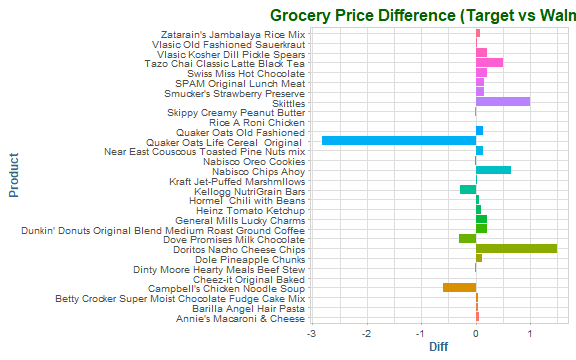
\includegraphics{03_permutation_testing_files/figure-latex/unnamed-chunk-34-1.png}

What is unusual about Quaker Oats Life cerial?

\textbf{Price difference is a multiple SD outlier.}

e.) Redo the hypothesis test without this observation.

\begin{Shaded}
\begin{Highlighting}[]
\NormalTok{diff <-}\StringTok{ }\NormalTok{Groceries[Product }\OperatorTok{!=}\StringTok{ "Quaker Oats Life Cereal  Original "}\NormalTok{, .(}\DataTypeTok{Diff =}\NormalTok{ Target }\OperatorTok{-}\StringTok{ }\NormalTok{Walmart ) ]}\OperatorTok{$}\NormalTok{Diff}

\NormalTok{observed <-}\StringTok{ }\KeywordTok{mean}\NormalTok{(diff)}

\NormalTok{N <-}\StringTok{ }\FloatTok{10e2} \OperatorTok{-}\StringTok{ }\DecValTok{1}
\NormalTok{results <-}\StringTok{ }\KeywordTok{numeric}\NormalTok{(N)}

\ControlFlowTok{for}\NormalTok{( i }\ControlFlowTok{in} \DecValTok{1}\OperatorTok{:}\NormalTok{N )}
\NormalTok{\{}
\NormalTok{   Sign <-}\StringTok{ }\KeywordTok{sample}\NormalTok{(}\KeywordTok{c}\NormalTok{(}\OperatorTok{-}\DecValTok{1}\NormalTok{, }\DecValTok{1}\NormalTok{), }\KeywordTok{length}\NormalTok{(diff), }\DataTypeTok{replace =}\NormalTok{ T)}
\NormalTok{   diff2 <-}\StringTok{ }\NormalTok{Sign }\OperatorTok{*}\StringTok{ }\NormalTok{diff}
\NormalTok{   results[i] <-}\StringTok{ }\KeywordTok{mean}\NormalTok{(diff2)}
\NormalTok{\}}

\NormalTok{p <-}\StringTok{ }\KeywordTok{min}\NormalTok{(}\DecValTok{1}\NormalTok{, }\DecValTok{2} \OperatorTok{*}\StringTok{ }\NormalTok{( }\KeywordTok{sum}\NormalTok{(results }\OperatorTok{>=}\StringTok{ }\NormalTok{observed ) }\OperatorTok{+}\StringTok{ }\DecValTok{1}\NormalTok{ ) }\OperatorTok{/}\StringTok{ }\NormalTok{( N }\OperatorTok{+}\StringTok{ }\DecValTok{1}\NormalTok{) )}
\end{Highlighting}
\end{Shaded}

Do you reach the same conclusion?

\textbf{No, there is a statistical difference in the prices of products
at the two retailers with the outlier removed.}

P-value: 0.036

\hypertarget{section-15}{%
\subsection{3.16}\label{section-15}}

In the sampling version of permutation testing, the one-sided P-value is

\(\hat{P} = \frac{(X + 1)}{(N + 1)}\), where X is the number of
permutation test statistics that are as large or larger than the
observed test statistic.

Suppose the true P-value (for the exaustive test, conditional on the
observed data) is \textbf{p}.

a.) What is the variance of \(\hat{P}\)?

\(\mathbb{V} = p*(1 - p) / (N + 1)\)

b.) What is the variance of \(\hat{P}_2\) for the two-sided test
(assuming that \textbf{p} is not close to 0.5, where \textbf{p} is the
smaller true one-side P-value)?

\end{document}
